% Formelsammlung Grundlagen elektrischer Maschinen
%
% Geschrieben im WS 2013/2014 an der TU München
% von Markus Hofbauer und Kevin Meyer für LaTeX4EI (latex4ei.de)
% Kontakt: latex@kevin-meyer.de oder via Kontaktformular auf http://latex4ei.de
% Aktuelle Versionen auf https://makeappdev.github.io/TUM-Projekte/

% Dokumenteinstellungen
% ======================================================================


% Dokumentklasse (Schriftgröße 6, DIN A4, Artikel)
\documentclass[fs, footer]{latex4ei}

\usepackage[european]{circuitikz}
\usepackage{tabularx}
\usepackage{multirow}
\usetikzlibrary{arrows, calc, intersections}
\usepackage{hyperref}
\urlstyle{sf}

% tabularx definition
\newcolumntype{C}{>{\centering\arraybackslash}X}
\newcolumntype{L}{@{\extracolsep\fill}X}

% SI-Zahlen mit Komma als Dezimaltrenner
\sisetup{locale=DE}
\sisetup{range-phrase = \ldots}
\sisetup{range-units = single}

% SI-Einheiten
\DeclareSIUnit \voltampere {VA}
\DeclareSIUnit \var {Var}
\DeclareSIUnit \newtonmeter {Nm}
\DeclareSIUnit \voltsecond {Vs}
\DeclareSIUnit \amperesecond {As}

% Nicht neuen, sondern alten Vector benutzen
\let\newvec = \vec
\let\vec = \oldvec

% Weitere Definitionen
\renewcommand{\ggT}[1]{\ensuremath{\operatorname{ggT}\left\{#1\right\}}}

% Eigener Inhalt für Center-Teil des Footers
\fancyfoot[C]{von Markus Hofbauer und Kevin Meyer - Kontakt: \href{mailto:latex@kevin-meyer.de}{\textit{latex@kevin-meyer.de}} - Homepage: \url{https://makeappdev.github.io/TUM-Projekte/}}

% Dokumentbeginn
% ======================================================================
\begin{document}

\IfFileExists{git.id}{\input{git.id}}{}
\ifdefined\GitRevision\fancyfoot[R]{Stand: \GitNiceDate \ (git \GitRevision) \qquad \thepage}\fi

% Aufteilung in Spalten
\begin{multicols*}{4}
\fstitle{Grundlagen elektrischer Maschinen}

\section{Grundlagen}
\sectionbox
{
\subsection{Größen}
\tablebox{
\begin{tabular*}{\columnwidth}{p{4.2cm}cc}
\ctrule
\multicolumn{3}{c}{\textbf{magnetische Größen}}\\
\cmrule
Durchflutung (magnetische Spannungsquelle) & $\Theta$ & $\unitof{\si{\ampere}}$\\
Fluss & $\Phi$ & $\unitof{\si{\voltsecond}}$\\
verketteter Fluss & $\Psi$ & $\unitof{\si{\voltsecond}}$\\
mag. Flussdichte & $\vec{B}$ & $\unitof{\si{\voltsecond\per\metre\squared}}$\\
mag. Feldstärke & $\vec{H}$ & $\unitof{\si{\ampere\per\metre}}$\\
magnetische Spannung & $V_m$ & $\unitof{\si{\ampere}}$\\
magnetischer Widerstand & $R_m$ & $\unitof{\si{\ampere\per\voltsecond}}$\\
Streuziffer & $\sigma$ & $\unitof{\si{1}}$\\
Remanenzflussdichte & $B_r$ & $\unitof{\si{\tesla}}$\\
kritische Feldstärke (aus Kennlinie ablesen) & $H_\text{M,krit}$ & $\unitof{\si{\ampere\per\meter}}$\\
Steigung Scherungsgerade & $k_\text{SG}$ & $\unitof{\si{1}}$\\
\cmrule
\multicolumn{3}{c}{\textbf{elektrische Größen}}\\
\cmrule
Stromdichte & $\vec{s}$ & $\unitof{\si{\ampere\per\metre\squared}}$\\
dielektrische Verschiebung & $\vec{D}$ & $\unitof{\si{\amperesecond\per\metre\squared}}$\\
el. Feldstärke & $\vec{E}$ & $\unitof{\si{\volt\per\metre}}$\\
Strombelag & $a$ & $\unitof{\si{\ampere\per\metre}}$\\
spezifischer Widerstand & $\rho$ & $\unitof{\si{\ohm\meter}}$\\
\cmrule
\multicolumn{3}{c}{\textbf{mechanische Größen}}\\
\cmrule
Drehmoment & $M$ & $\unitof{\si{\newtonmeter}}$\\
Massenträgheitsmoment & $J$ & $\unitof{\si{\kilo\gram\metre\squared}}$\\
Spulenwindungszahl & $w_\text{Sp}$ & $\unitof{1}$\\
effektive Windungszahl & $w_\text{eff}$ & $\unitof{\si{1}}$\\
Luftspalthöhe & $\delta$ & $\unitof{\si{\milli\meter}}$\\
scheinbarer Luftspalt & $\delta'$ & $\unitof{\si{\milli\meter}}$\\
effektiver Luftspalt & $\delta''$ & $\unitof{\si{\milli\meter}}$\\
Anzahl der Leiter pro Nut & $Z_\text{N}$ & $\unitof{\si{1}}$\\
Zahl der Einzelspulen (Kommutatorsegmente) & $Z_K$ & $\unitof{\si{1}}$\\
ideelle Eisenlänge & $l_i$ & $\unitof{\si{\meter}}$\\
bewickelbare Nutfläche & $A_N$ & $\unitof{\si{\meter\squared}}$\\
magnetisch aktiver Winkel & $\beta_M$ & $\unitof{\si{\radian}}$\\
Drehzahl & $n$ & $\unitof{\si{\per\second}}$\\
Rotornutenzahl & $N$ & $\unitof{\si{1}}$\\
Rotornutenzahl pro Pol & $Q$ & $\unitof{\si{1}}$\\
Anzahl paralleler Zweige & $a$ & $\unitof{\si{1}}$\\
\cmrule
\multicolumn{3}{c}{\textbf{Näherungsfaktoren}}\\
\cmrule
Carterfaktor & $k_\text{C}$ & $\unitof{\si{1}}$\\
Eisenfüllfaktor & $k_\text{Fe}$ & $\unitof{\si{1}}$\\
Eisenfaktor (Magnnetisierungsbedarf Eisen) & $k_\mu$ & $\unitof{\si{1}}$\\
Nutfüllfaktor & $k_Q$ & $\unitof{\si{1}}$\\
Sicherheitsfaktor & $\gamma_\text{krit}$ & $\unitof{\si{1}}$\\
\cbrule
\end{tabular*}
}
}
\sectionbox{
\symbolbox{
\begin{tabularx}{\columnwidth}{lX}
Permeabilität & $\mu_0 = \SI{4\pi e-7}{\volt\second\per\ampere\metre}$ \\
Permittivität & $\varepsilon_0 = \SI{8,854e-12}{\ampere\second\per\volt\metre}$
\end{tabularx}
}
\subsubsection{Allgemeine Maschinenbegriffe - Durchmesser}
\mbox{
\pbox[c]{4cm}{
    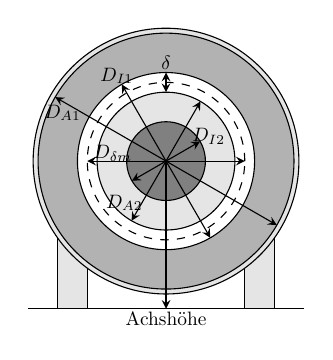
\begin{tikzpicture}[scale=.5,every node/.style={scale=.7} , >=stealth]
	\draw (-3.5,-3.75) -- (3.5,-3.75);

	\filldraw[fill=black!10!white, draw=black]
		(-2.75,-3.75) rectangle (-2.0,0);
	\filldraw[fill=black!10!white, draw=black]
		(2.75,-3.75) rectangle (2.0,0);
	
	\filldraw[fill=black!10!white, draw=black]
		(0,0) circle (3.375 cm);
	\filldraw[fill=black!30!white, draw=black]
		(0,0) circle (3.25 cm);
	\filldraw[fill=white, draw=black]
		(0,0) circle (2.25 cm);
	\draw [dashed] (0,0) circle (2.0 cm);
	\filldraw[fill=black!10!white, draw=black]
		(0,0) circle (1.75 cm);
	\filldraw[fill=black!50!white, draw=black]
		(0,0) circle (1 cm);
		
	% Achshöhe
	\draw [->] (0,0) -- (0,-3.75);
	\draw (0, -4) node {Achshöhe}; 
	
	% D_\delta m
	\draw [<->] (-2,0) -- (2,0); 
	\draw (-1.35,0.2) node {$D_{\delta\text m}$};

	% delta
	\draw [<->] (0,1.75) -- (0,2.25);
	\draw (0,2.5) node {$\delta$};

	% D_I2
	\draw [<->] (210:1) -- (30:1);
	\draw (30:1.25) node {$D_\text{I2}$};

	% D_A1
	\draw [<->] (150:3.25) -- (330:3.25);
	\draw (155:2.9) node {$D_\text{A1}$};
	
	% D_A2
	\draw [<->] (60:1.75) -- (240:1.75);
	\draw (225:1.5) node {$D_\text{A2}$}; 

	% D_I1
	\draw [<->] (120:2.25) -- (300:2.25);
	\draw (120:2.5) node {$D_\text{I1}$}; 
	
\end{tikzpicture}
	}
	}
\begin{minipage}{3cm}
	\tablebox{
	\begin{tabularx}{\columnwidth}{l c}
		\ctrule
		\multicolumn{2}{c}{\textbf{Maße}}\\
		\cmrule
		Stator Außend. & $D_\text{A1}$\\
		Stator Innend. & $D_\text{I1}$\\
		Rotor Außend. & $D_\text{A2}$\\
		Rotor Innend. & $D_\text{I2}$\\
		\cmrule
		\multirow{2}{*}{Mittl. Luftspaltd.} & $D$\\
		& $D_{\delta\text m}$\\
		\cmrule
		Luftspalthöhe & $\delta$\\
		\cbrule
	\end{tabularx}
	}
\end{minipage}

\subsubsection{Allgemeine Maschinenbegriffe - Abmessungen}
\mbox{
\pbox[c]{4cm}{
    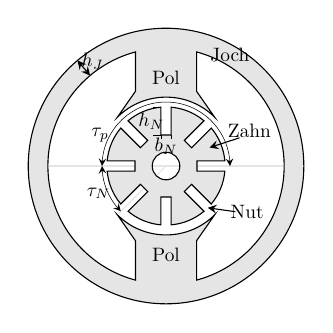
\begin{tikzpicture}[scale=.5,every node/.style={scale=.7} , >=stealth]
	
	\filldraw[fill=black!10!white, draw=black] 
		(0,0) circle (3.5 cm);
	
	\filldraw[fill=white, draw=black] 
		(105:3.0) arc (105:255:3.0) 
		-- ++(0,1) -- (225:1.75) arc (225:315:1.75) 
		-- ($(285:3.0) + (0,1)$) -- ++(0,-1) arc (-75:75:3.0) 
		-- +(0,-1) -- (45:1.75) arc (45:135:1.75)
		-- ($(105:3.0) + (0,-1)$) -- cycle;

	\draw[draw=black!10!white]
		(-2.98,0) -- (2.98,0);
	
	\draw[draw=black!10!white]
		(0,0) -- (225:1.73);
	
	\coordinate (a1) at (5:1.5);
	\coordinate (i1) at ($(5:1.5) + (-0.707,0)$);
	\coordinate (i2) at ($(40:1.5) + (-0.5,-0.5)$);
	\coordinate (i3) at ($(50:1.5) + (-0.5,-0.5)$);
	\coordinate (i4) at ($(85:1.5) - (0,0.707)$);
	\coordinate (i5) at ($(95:1.5) - (0,0.707)$);
	\coordinate (i6) at ($(130:1.5) - (-0.5,0.5)$);
	\coordinate (i7) at ($(140:1.5) - (-0.5,0.5)$);
	\coordinate (i8) at ($(175:1.5) - (-0.707,0)$);
	\coordinate (i9) at ($(185:1.5) - (-0.707,0)$);
	\coordinate (i10) at ($(220:1.5) - (-0.5,-0.5)$);
	\coordinate (i11) at ($(230:1.5) - (-0.5,-0.5)$);
	\coordinate (i12) at ($(265:1.5) - (0,-0.707)$);
	\coordinate (i13) at ($(275:1.5) - (0,-0.707)$);
	\coordinate (i14) at ($(310:1.5) - (0.5,-0.5)$);
	\coordinate (i15) at ($(320:1.5) - (0.5,-0.5)$);
	\coordinate (i16) at ($(355:1.5) - (0.707,0)$);
	\coordinate (b1) at ($(85:1.5) - (0,0.8)$);
	\coordinate (b2) at ($(95:1.5) - (0,0.8)$);
	
	\filldraw[fill=black!10!white, draw=black] 
		(i1) -- (a1) 
		arc (5:40:1.5) -- (i2) -- (i3) -- ++(0.5,0.5) 
		arc (50:85:1.5) -- (i4) -- (i5) -- ++(0,0.707)
		arc (95:130:1.5) -- (i6) -- (i7) -- ++(-0.5,0.5)
		arc (140:175:1.5) -- (i8) -- (i9) -- ++(-0.707,0)
		arc (185:220:1.5) -- (i10) -- (i11) -- ++(-0.5,-0.5)
		arc (230:265:1.5) -- (i12) -- (i13) -- ++(0,-0.707)
		arc (275:310:1.5) -- (i14) -- (i15) -- ++(0.5,-0.5)
		arc (320:355:1.5) -- (i16) -- cycle;

	\filldraw[fill=white, draw=black]
		(0,0) circle (0.35cm);

	% h_j
	\draw [<->] (130:3.5) -- (130:3);
	\draw (125:3.25) node {$h_\text{J}$};  
	
	% Beschriftung
	\draw (60:3.25) node {Joch};
	\draw (0, 2.25) node {Pol};
	\draw (0, -2.25) node {Pol};
	
	\draw [<-] (23:1.2) -- (21:2.0);
	\draw (23:2.3) node {Zahn};
	
	\draw [<-] (315:1.5) -- ++(0.7,-0.1);
	\draw (315:1.5) ++(0.7,-0.1) ++(0.3,0) node {Nut};
	
	% Hilfslinien
	\draw[draw=black!10!white]
		(-0.33,0) -- (0.33,0);
	\draw[draw=black!10!white]
		(0,0) -- (225:0.33);
	
	% tau_N
	\draw [<->, very thin] (180:1.625) arc (180:225:1.625);
	\draw (202:1.85) node {$\tau_\text N$};

	% tau_p
	\draw [<->, very thin] (0:1.625) arc (0:180:1.625);
	\draw (155:1.85) node {$\tau_p$};
	
	% b_N
	\draw [very thin] (i4) -- (b1);
	\draw [very thin] (i5) -- (b2);
	\draw (0,0.5) node {$b_\text{N}$};	
	
	% h_N
	\draw [very thin] (95:1.5) -- +(-0.2,0);
	\draw [very thin] (i5) -- +(-0.2,0);
	\draw (108:1.2) node {$h_\text{N}$};
	
	
\end{tikzpicture}
	}
	}
\begin{minipage}{3cm}
	\tablebox{
	\begin{tabularx}{\columnwidth}{l c c}
		\ctrule
		\multicolumn{3}{c}{\textbf{Maße}}\\
		\cmrule
		Nutzahl & $N$ & $\unitof{\si{1}}$\\
		Nutteilung & $\tau_\text{N}$ & $\unitof{\si{\centi\metre}}$\\
		\cmrule
		Polpaarzahl & $p$ & $\unitof{\si{1}}$ \\
		Polteilung & $\tau_\text{p}$ & $\unitof{\si{\centi\metre}}$\\
		\cmrule
		Nuthöhe & $h_\text{N}$ & $\unitof{\si{\centi\metre}}$\\
		Nutbreite & $b_\text{N}$ & $\unitof{\si{\centi\metre}}$\\
		Jochhöhe & $h_\text{J}$ & $\unitof{\si{\centi\metre}}$\\
		\cbrule
	\end{tabularx}
	\begin{tabularx}{\columnwidth}{c c}
		\ctrule
		$\tau_\text{N} = \frac{\pi\cdot D}{N}$ & $\tau_\text{p} = \frac{\pi\cdot D}{2p}$\\
		\cbrule
	\end{tabularx}
	}
\end{minipage}
}
\sectionbox{
\subsection{Grundlegende Gleichungen}
\subsubsection{Maxwell}

\begin{tabularx}{\columnwidth}{>{\centering\arraybackslash}m{0.435\columnwidth}|>{\centering\arraybackslash}m{0.435\columnwidth}}
$\rot \vec{H} = \vec{s} + \frac{\partial\vec{D}}{\partial t}$  & \multirow{2}{*}{$\rot\vec{E} = - \frac{\partial\vec{B}}{\partial t}$} \\
$\rot \vec{H} = \vec{s} \quad (< 10\si{\kilo\hertz})$ & \\
\hline
\multirow{2}{*}{$\div\vec B = 0$} & \multirow{2}{*}{$\div\vec D = \gamma$} \\
 & \\
\end{tabularx}

\subsubsection{Durchflutungs- und Induktionsgesetz}
\begin{tabularx}{\columnwidth}{>{\centering\arraybackslash}m{0.435\columnwidth}|>{\centering\arraybackslash}m{0.435\columnwidth}}
\textbf{Durchflutungsgesetz} & \textbf{Induktionsgesetz}\\
\hline
\vspace{3pt}$\oint_{L_\text{A}}\vec{H}\diff\vec{l} = \iint_{A_\text{L}}\vec{s}\diff\vec{A} = \Sigma i = \Theta$ & \vspace{3pt}\mbox{$u_i = \frac{\partial\Psi(t)}{\partial t} = \frac{\partial}{\partial t}\left(\iint_A \vec{B}\diff\vec{A}\right)$}
$\oint_L \vec{E}\diff\vec{l} + u_\text{i} = 0$\\
\end{tabularx}

\subsubsection{Kenngrößen}
\begin{tabularx}{\columnwidth}{>{\centering\arraybackslash}m{0.435\columnwidth}|>{\centering\arraybackslash}m{0.435\columnwidth}}
\textbf{magnetische Größen} & \textbf{elektrische Größen}\\
\hline
\vspace{3pt}$\Phi = \iint\vec{B}\diff\vec{A}$ & \vspace{3pt}$I = \iint\vec{s}\diff\vec{A}$\\
$V_m = \int \vec{H}\diff\vec{l}$ & $U = \int \vec{E}\diff\vec{l}$\\
$\Theta = w\cdot I$ & \\
$R_m = \frac{V_m}{\Phi} = \frac{l}{\mu\cdot A}$ & $R = \frac{U}{I} = \rho\frac{l}{A}$\\
$\vec{B} = \mu\cdot\vec{H}$ & $\vec{D} = \varepsilon\cdot \vec{E}$\\
$\Psi = \Phi\cdot w = L\cdot i$ & \\
\vspace{3pt}
\begin{circuitikz}[scale=.8, transform shape, font=\large]
\draw	(0,2) to [short, i=$\Phi$] (1.5,2)
			to [R, l_=$R_\text{m}$,v^>=$V$](1.5,0)
			to (0,0)
			to [V<=$\Theta$](0,2);
\end{circuitikz} & \vspace{3pt}
\begin{circuitikz}[scale=.8, transform shape, font=\large]
\draw	(4,2) to [short, i=$I$] (5.5,2)
			to [R, l_=$R$,v^>=$U$](5.5,0)
			to (4,0)
			to [V<=$U$](4,2);
\end{circuitikz}\\
magnetisch wirksame Fläche & \\
$A = k_\text{Fe}\cdot A_\text{geometrisch}$
\end{tabularx}
}
\sectionbox{
\subsection{Entstehung des Drehmoments}
\subsubsection{Lorenzkraft}

\[\vec{F_\text{L}} = I\cdot (\vec{l}\times \vec{B})\]

\subsubsection{Drehmoment}
\emphbox{$M_\text{D} = F\cdot r = M_L + M_R + J\frac{\diff\omega}{\diff t}$}
\[m_d(t) = \left(\frac{D}{2}\right)^2\cdot\int_{-\frac{l_i}{2}}^{\frac{l_i}{2}}\int_{0}^{2\pi}a(\vartheta,z,t)B_\delta(\vartheta,z,t)\diff\vartheta\diff z\]

\subsubsection{Strombelag}
\begin{align*}
a = \int\vec{s}\diff\vec{l} = \frac{\partial\sum i}{\partial l} = \frac{\partial}{\partial l}\left[\iint_A \vec{s}\diff\vec{A}\right] = -\frac{\partial\Theta}{\partial l}
\end{align*}
\begin{tabularx}{\columnwidth}{>{\centering\arraybackslash}X >{\centering\arraybackslash}X}
mittlerer Strombelag & Amplitude\\
$a_m = \frac{b_\text{N}}{\tau_\text{N}}\cdot A_\text{N} = \frac{\sum\Theta_\text{N}}{\tau_p}$ & $A_\text{N} = \frac{Z_\text{N}\cdot i}{b_\text{N}} = \frac{\Theta_\text{N}}{b_\text{N}}$
\end{tabularx}

\subsubsection{Felderregerkurve}
\[V(\vartheta) = \Theta(\vartheta) = -\frac{D}{2}\int a_\text{ges}(\vartheta)\diff\vartheta\]
}
\sectionbox{
\subsection{Effektiver Luftspalt}
Magnetfeld wegen Nuten inhomogen. Ausgleich durch Carterfaktor $k_\text{C}$ (ungenutet $k_\text{C,i} = 1$):\\
\begin{tabular}{lll}
$\delta' = k_\text{C}\cdot\delta$ & $k_\text{C} = \underset{\text{Stator}}{k_\text{C1}}\cdot \underset{\text{Rotor}}{k_\text{C2}}$ & $k_\text{C,i} = \frac{\tau_\text{N,i}}{\tau_\text{N,i} -\gamma_i \cdot\delta}$\\\\
$\delta'' = k_\mu\cdot k_\text{Abfl}\cdot\delta'$ &
$\gamma_i = \frac{\left(\frac{b_\text{N,i}}{\delta}\right)^2}{5+\left(\frac{b_\text{N,i}}{\delta}\right)}$ &
$\tau_\text{N,i} = \frac{\pi\cdot D}{N_i}$\\
$k_\mu = 1 + \frac{V_{m\text{Fe}}}{2\cdot V_{m\delta'}}$ & &
\end{tabular}
}
\sectionbox{
\subsection{Streuung}
\subsubsection{Polstreuung}
\begin{minipage}{0.7\columnwidth}
$\Phi_\text{E}$: Gesamtfluss durch Polspule \\
$\Phi_\text{Eh}$: Hauptfluss \\
$\Phi_{\text{E}\sigma}$: Streufluss
\end{minipage}
\begin{minipage}{0.25\columnwidth}
$\sigma_\text{E} = \frac{\Phi_{\text{E}\sigma}}{\Phi_\text{Eh}}$
\end{minipage}
$\Phi_\text{E} = \Phi_\text{Eh} + \Phi_{\text{E}\sigma} = (1+\sigma_\text{E})\cdot \Phi_\text{Eh}$
\\
\subsubsection{Nut- und Zahnkopfstreuung}
\begin{minipage}{0.7\columnwidth}
$\Phi_N$: Gesamtfluss der in Nuten gebetteten Spulen\\
$\Phi_\text{Nh}$: Hauptfluss\\
$\Phi_{\text{N}\sigma}$: Streufluss (Nut- \& Zahnkopfstreuung)
\end{minipage}
\begin{minipage}{0.25\columnwidth}
$\sigma_\text{N}=\frac{2 \cdot \Phi_{\text{N}\sigma}}{\Phi_\text{Nh}}$
\end{minipage}
$\Phi_\text{N} = \Phi_\text{Nh} + 2\Phi_{\text{N}\sigma} = (1 + \sigma_\text{N})\cdot\Phi_\text{Nh}$
\\
\subsubsection{Stirnstreuung}
\begin{minipage}{0.7\columnwidth}
$\Phi_\text{S}$: Gesamtfluss Stirnstreuung\\
$\Phi_\text{Sh}$: Hauptfluss Stirnstreuung\\
$\Phi_{\text{S}\sigma}$: Streufluss Stirnstreuung
\end{minipage}
\begin{minipage}{0.25\columnwidth}
$\sigma_\text{S}=\frac{\Phi_{\text{S}\sigma}}{\Phi_\text{Sh}}$
\end{minipage}
gesamte Streuziffer: $\sigma_\text{ges}=\frac{\Phi_{\sigma, \text{ges}}}{\Phi_\text{Sh}}$\\
$\Phi_\text{S} = \Phi_\text{Sh} + \Phi_{\sigma,\text{ges}} = (1+\sigma_\text{ges})\cdot \Phi_\text{Sh}$
\\
\subsubsection{Induktivitäten}
Hauptinduktivität: $L_\text{h}=\frac{\Psi_\text{h}}{i}$\\
Gesamte Streuinduktivität: $L_{\sigma}=\frac{\Psi_{\sigma}}{i}=\sigma \cdot L_\text{h}$ \\
Totale Induktivität: $L_\text{ges}= \frac{\Psi_\text{ges}}{i}=(1+\sigma) \cdot L_\text{h}$
}
\sectionbox{
\subsection{Spulen}
\begin{tabularx}{\columnwidth}{lX}
Spulenwindungszahl & $w_\text{Sp} = \frac{Z_\text{N}}{2 \cdot u}$\\
Nebeneinanderliegende Spulenseiten pro Nut & $u = \frac{Z_K}{N}$\\
Wellenwicklung & $a = 2$\\
Schleifenwicklung & $a = 2\cdot p$
\end{tabularx}
}
\sectionbox{
\subsection{Verluste}
\subsubsection{Kupferverluste}
\begin{center}
\fbox{$P_\text{Cu}=R \cdot I^2$}
\end{center}

\subsubsection{Reibungsverluste}
\begin{itemize}
\item Ventilationsverluste (Verwirbelung im Kühlmittel, Strömungsverluste)
\item Lagerreibung
\item Reibung an Kontaktflächen (z.B Schleifringe, Kommutator)
\end{itemize}

\subsubsection{Hystereseverluste}
$P_\text{FeH}=m_\text{Fe} \cdot v_{15\text{H}} \cdot \frac{f}{\SI{50}{\hertz}} \cdot (\frac{B}{\SI{1,5}{\tesla}})^2$\\
Verlustziffer: $v_{15\text{H}}(f=15\si{\hertz},B=\SI{1,5}{\tesla})\unitof{\si{\watt\per\kilo\gram}}$ (Herstellerangabe)

\subsubsection{Wirbelstromverluste}
$P_\text{FeW}=m_\text{Fe} \cdot v_{15\text{W}} \cdot (\frac{f}{\SI{50}{\hertz}})^2 \cdot (\frac{B}{\SI{1,5}{\tesla}})^2$\\
Verlustziffer: $v_{15\text{W}}(f=15\si{\hertz},B=\SI{1,5}{\tesla})\unitof{\si{\watt\per\kilo\gram}}$ (Herstellerangabe)

\subsubsection{Gesamte Eisenverluste}
$P_\text{Fe}=m_\text{Fe} \cdot v_{\text{Fe}15} {\cdot} \frac{f}{\SI{50}{\hertz}}\cdot(\frac{B}{\SI{1,5}{\tesla}})^2$\\

\subsection{Leistung}
\subsubsection{mechanische Leistung}
\emphbox{$P_m = 2\pi\cdot n\cdot M_i = \omega_m\cdot M_i$}

\subsubsection{elektrische Leistung}
\emphbox{$P_\text{el} = U\cdot I$}

\subsection{Wirkungsgrad}
\emphbox{$\eta = \frac{P_\text{ab}}{P\text{auf}}$}
\begin{tabularx}{\columnwidth}{>{\centering\arraybackslash}X >{\centering\arraybackslash}X}
$\eta_\text{Motor} = \frac{P_m}{P_\text{el}}$ & $\eta_\text{Generator} = \frac{P\text{el}}{P_m}$
\end{tabularx}
}

\section{Gleichstrommaschine}
\sectionbox{
\subsection{Größen}
\tablebox{
\begin{tabular*}{\columnwidth}{p{4,5cm}cc}
\ctrule
Maschinenkonstante (Spannung) & $k_U$ & $\unitof{\si{1}}$\\
Maschinenkonstante (Drehmoment) & $k_M$ & $\unitof{\si{1}}$\\
Flusskonstante & $k_\Phi$ & $\unitof{\si{\voltsecond\per\ampere}}$\\
Erregerstromkonstante & $k_E$ & $\unitof{\si{1}}$\\
Ankerwindungszahl & $w_2$ & $\unitof{\si{1}}$\\
Bürstenübergangsspannung & $U_B$ & $\unitof{\si{\volt}}$\\
Kommutatorsegmentspannung & $U_S$ & $\unitof{\si{\volt}}$\\
\cbrule
\end{tabular*}
}
\subsection{Systemgleichungen}
\begin{align*}
U_A &= R_{A,\text{res}}\cdot I_A + U_i + 2\cdot U_B & w_2 = \frac{N_2 \cdot Z_N}{2a}\\
\Phi_E &= k_\Phi\cdot I_E & k_U = 4p\cdot w_2\\
U_i &= k_U\cdot\Phi_E\cdot n & k_M = \frac{k_U}{2\pi}\\
M_i &= k_M\cdot\Phi_E\cdot I_A\\
M_i &= M_R + M_L + J\frac{\diff\omega}{\diff t}
\end{align*}

\subsection{Verhalten}
\begin{center}
%!tikz editor 1.0
%!tikz source begin
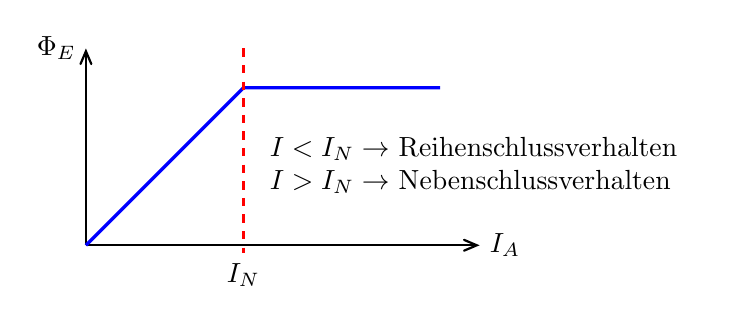
\begin{tikzpicture} [>=angle 45]

% Koordinatensystem
\draw [->, thick] (0, 0) -- (5, 0) node [right] {$I_A$};
\draw [->, thick] (0, 0) -- (0, 2.5) node [left] {$\Phi_E$};

\coordinate (P1) at (2, 2);
\coordinate (P2) at (4.5, 2);

\draw [blue, very thick] (0,0) -- (P1) -- (P2);
\draw [red, dashed, thick] (2, 2.5) -- (2, -0.1) node [below, black] {$I_N$};
\draw (2,1) node [right] {\begin{tabular}{l} $I < I_N \rightarrow$ Reihenschlussverhalten \\ $I > I_N \rightarrow$ Nebenschlussverhalten\end{tabular}};


\end{tikzpicture}
%!tikz source end

\end{center}
}
\sectionbox{
\subsection{Gleichstrom-Nebenschlussmaschine}
\subsubsection{ESB}
\begin{center}
\begin{circuitikz}[scale=.75, transform shape, font=\large]
\draw[american currents]
	(0,2)
	to [short, i=$I_A$, o-]	(0.5,2) 
	to [R=$R_A$]		(2,2)
	to [L=$L_A$]			(4,2)
	to [I_=$U_i$]		(4,0)
	to [I=$U_B$] (2,0)
	to [short, -o]		(0,0);
\draw[->, >=latex] (0,1.8) -- (0,0.2) node [pos=0.5, left] {$U_A$};
\draw
	(6,0.5) 
	to [short, o-]		(6,1)
	to [R=$R_E$]			(8,1)
	to [short, i=$I_E$, -o]		(8,0.5);
\draw[->, >=latex] (6.2,0.5) -- (7.8,0.5) node [pos=0.5, below] {$U_E$};
\draw[->, >=latex]
	(4.8,1) -- (5.5,1);
\draw	
	(5.1,1.25) node {$\Phi_E$};
\end{circuitikz}
\end{center}

\subsubsection{Drehmoment-Drehzahl-Kennlinie}
\emphbox{
\[n = \frac{U_A - 2\cdot U_B}{k_U\cdot\Phi_E} - \frac{2\pi\cdot R_{A,\text{res}}}{(k_U\cdot\Phi_E)^2}\cdot M_i\]
}

\subsubsection{Wichtige Betriebspunkte}
\begin{align*}
&\text{Anlaufmoment: } (n = 0) & M_{i,\text{An}} &= k_M\cdot\Phi_E\cdot I_{A,\text{An}}\\
&\text{Leerlaufdrehzahl: } (M_i = 0) & n_0 &= \frac{U_A - 2\cdot U_B}{k_U\cdot\Phi_E}\\
&\text{Anlaufstrom: } (n = 0) & I_{A,\text{An}}& = \frac{U_A - 2\cdot U_B}{R_{A,\text{res}}}\\
&n = n_0\cdot\left(1 - \frac{M_i}{M_{i,\text{An}}}\right) & M_i &= M_{i,\text{An}}\cdot\left(1 - \frac{n}{n_0}\right)
\end{align*}
}
\sectionbox{
\subsection{Gleichstrom-Reihenschlussmaschine}
\subsubsection{ESB}
\begin{center}
\begin{circuitikz}[scale=.9, transform shape]
\draw [american currents]
	(0,3) to [short, i=$I_A$, o-]
	(0.5, 3)
	(2,3) to [vR, l_=$R_V$]
	(0.5,3)
	(2,3) to [R=$R_A$]
	(3.5,3) to [L=$L_{EH}$]
	(5,3) to [L=$L_{E\sigma}$]
	(6.5,3) to [I=$U_B$]
	(6.5,1.5) to [I=$U_i$]
	(6.5,0) to [short]
	(5.5,0) to [L=$L_{A\sigma}$]
	(4,0) to [L=$L_{AH}$]
	(2.5,0) to [R=$R_E$, i=$I_E$]
	(0.5,0) to [short, -o]
	(0,0);
	
\draw[->, >=latex] (0,2.8) -- (0,0.2) node [pos=0.5, right] {$U_A$};
\draw
	(5.8,0)
	to [short, *-] (5.8,1)
	to [R=$R_P$] (0.5,1)
	to [short, -*] (0.5,0);
\end{circuitikz}

\end{center}
\begin{align*}
R_{A,\text{res}} &= R_V + R_A + R_E || R_P
\end{align*}

\subsubsection{Systemgleichungen}
\begin{align*}
I_E &= k_E\cdot I_A \quad\text{mit } k_E =
\begin{cases}
1 & \text{für } R_P \rightarrow\infty\\
0 & \text{für } R_P =0\\
\dfrac{R_p}{R_p + R_E} & \text{sonst}
\end{cases}\\
\Phi_E &= k_\Phi\cdot I_E = k_\Phi\, k_E\cdot I_A\\
M_i & = k_M \cdot \Phi_E \cdot I_A = k_M \, k_\Phi \, k_E \cdot {I_A}^2\\
U_i & = k_U \cdot \Phi_E \cdot n = k_U \, k_\Phi \, k_E \cdot I_A \cdot n\\
\end{align*}
}
\sectionbox{
\subsubsection{Drehmoment-Drehzahl-Kennlinie}
\emphbox{
\[M_i = k_M\, k_\Phi\, k_E\cdot\frac{(U_A - 2\cdot U_B)^2}{(k_U\, k_\Phi\, k_E\cdot n + {R_{A,\text{res}}}^2)^2} \]
}
\begin{align*}
\text{Anlaufmoment: }(n=0)\qquad M_{i,\text{An}} = k_M\, k_\Phi\, k_E\cdot\left(\frac{U_A}{R_{A,\text{res}}}\right)^2
\end{align*}
}
\sectionbox{
\subsection{Permanenterregte Gleichstrommaschine}
\subsubsection{ESB}
\centerline{
\begin{circuitikz}[scale=.75, transform shape, american currents] 
\draw	(0,2) to [R=$R_A$, o-]
		(2,2) to [L=$L_A$]
		(4,2) to [I=$U_B$]
		(6,2) to [I_=$U_I$]
		(6,0) to [short, -o] (0,0);

\draw[->, >=latex] (0,1.8) -- (0,0.2) node [pos=0.5, left] {$\underline U_1$};
\draw (6.8,1.1) rectangle (7.5,0.9);
\draw [fill=black] (7.5,1.1) rectangle (8.2,0.9);
\end{circuitikz}
}
\subsubsection{Systemgleichungen}
\begin{tabularx}{\columnwidth}{LX}
Maximaler Ankerstrom: & $I_\text{A,max} = I_L \cdot a = S \cdot A_L \cdot a$\\
Maximale Ankerspannung: & $U_\text{A,max} = U_S \cdot \frac{Z_K}{2\cdot p}$
\end{tabularx}
}

\section{Wechselfeld - Drehfeld}
\sectionbox{
\subsection{Größen}
\tablebox{
\begin{tabular*}{\columnwidth}{p{4,5cm}cc}
\ctrule
Stator & Index 1 & \\
Rotor & Index 2 & \\
Ordnungszahl der Oberwellen & $\nu$ & $\unitof{\si{1}}$\\
\cmrule
elektrische Frequenz & $f$ & $\unitof{\si{\hertz}}$\\
elektrische Kreisfrequenz & $\omega$ & $\unitof{\si{\radian\per\second}}$\\
\multicolumn{3}{c}{$\omega = 2\pi f$}\\
mechanische Kreisfrequenz & $\omega_m$ & $\unitof{\si{\radian\per\second}}$\\
Phasenwinkel & $\varphi$ & $\unitof{\si{\radian}}$\\
Strangachsenwinkel & $\vartheta$ & $\unitof{\si{\radian}}$\\
Strangspannung & $U_1$ & $\unitof{\si{\volt}}$\\
Strangstrom & $I_1$ & $\unitof{\si{\ampere}}$\\
komplexe Scheinleistung & $\underline{S}$ & $\unitof{\si{\voltampere}}$\\
Wirkleistung & $P$ & $\unitof{\si{\watt}}$\\
Blindleistung & $Q$ & $\unitof{\si{\var}}$\\
Strangzahl & $m$ & $\unitof{\si{1}}$\\
Windungszahl pro Strang & $w_1$ & $\unitof{\si{1}}$\\
\cmrule
Lochzahl (Nuten pro Pol und Strang) & $q$ & $\unitof{\si{1}}$\\
Nutwinkel & $\alpha_N$ & $\unitof{\si{\radian}}$\\
Spulenwinkel & $\alpha_\text{Sp}$ & $\unitof{\si{\radian}}$\\
Polwinkel & $\alpha_p$ & $\unitof{\si{\radian}}$\\
Spulenweite & $W_\text{Sp}$ & $\unitof{\si{\centi\meter}}$\\
Zonungsfaktor & $\xi_Z$ & $\unitof{\si{1}}$\\
Sehnungsfaktor & $\xi_S$ & $\unitof{\si{1}}$\\
Nutschlitzbreitenfaktor & $\xi_N$ & $\unitof{\si{1}}$\\
Schrägungsfaktor & $\xi_\text{Schr}$ & $\unitof{\si{1}}$\\
\cbrule
\end{tabular*}
}
}
\sectionbox{
\subsection{Stern \& Dreieckschaltung}
\emphbox{
\begin{tabularx}{\columnwidth}{>{\centering\arraybackslash}X |>{\centering\arraybackslash}X}
\textbf{Sternschaltung} & \textbf{Dreiecksschaltung}\\
$U_1 = \frac{U_N}{\sqrt{3}}$ & $U_1 = U_N$\\
$I_1 = I_N$ & $I_1 = \frac{I_N}{\sqrt{3}}$\\
\end{tabularx}
}
}
\sectionbox{
\subsection{Allgemeines zu Wechselgrößen}
\symbolbox{
\begin{tabularx}{\columnwidth}{>{\centering\arraybackslash}X>{\centering\arraybackslash}X}
$\underline{a}^\nu = e^{j\nu\frac{2\pi}{3}}$ & $\underline{a}^0 + \underline{a}^1 + \underline{a}^2 = 0$\\
\multicolumn{2}{c}{$\underline{a}^2 = \underline{a}^* = e^{j\frac{4\pi}{3}} = e^{-j\frac{2\pi}{3}}$}
\end{tabularx}
}
\begin{align*}
x(t) &= \sqrt{2}\cdot X\cdot\cos(\omega t + \varphi)\\
\vec{x}(t) &= \frac{1}{3}\cdot\left[x_A(t) + \newvec{a}\cdot x_B(t) + \newvec{a}^2\cdot x_C(t) \right] = \frac{\sqrt{2}}{2}\cdot\underline X\cdot e^{j\omega t}\\
\underline{X} &= X\cdot e^{j\varphi}
\end{align*}

\subsubsection{Wechselfeld}
\begin{align*}
B(\vartheta,t) = \hat{B}\cdot\cos(\vartheta - \vartheta_0)\cdot\cos(\omega t - \varphi)
\end{align*}

\subsubsection{Drehfeld}
\begin{align*}
B(\vartheta,t) = \hat{B}\cdot\cos((\vartheta - \vartheta_0) - (\omega t - \varphi))
\end{align*}
}
\sectionbox{
\subsection{Einfluss realer Luftspalt}
\label{subsec:wickl}
\symbolbox{Wicklungsfaktor: $\qquad\xi_{(\nu)} = \xi_{Z(\nu)}\cdot\xi_{S(\nu)}\cdot\xi_{N(\nu)}$}
\[w_\text{eff} = w_\text{Sp}\cdot\xi_{(\nu)}\]
\begin{tabularx}{\columnwidth}{cCc}
$\alpha_N = \frac{2\pi}{N}$ & $\alpha_\text{Sp} = W_\text{Sp}(\text{absolut})\cdot\alpha_N$ & $\alpha_p = \frac{2\pi}{2p}$
\end{tabularx}

\subsubsection{Zonung}
Erhöhung der Lochzahl $q$\\
(Beschränkt durch $N_\text{max} = \frac{D\pi}{\tau_{N,\text{min}}}$) mit $\tau_{N,\text{min}} \approx \SI{1}{\centi\meter}$
\begin{align*}
w_\text{eff} &= q\cdot w_\text{Sp}\cdot\xi_{Z(\nu)}\\
\xi_{Z(\nu)} &= \frac{\sin\left(q\cdot\nu\frac{\alpha_N}{2}p\right)}{q\cdot\sin\left(\nu\frac{\alpha_N}{2}p\right)} = \frac{\sin\left(\nu\frac{\pi}{2}\frac{q}{Q}\right)}{q\cdot\sin\left(\nu\frac{\pi}{2}\frac{1}{Q}\right)}
\end{align*}

\subsubsection{Sehnung}
Kürzung der Spulenweite $W_\text{Sp}$ (nicht bei Einschichtwicklung möglich)\\
\begin{align*}
w_\text{eff} &= q\cdot w_\text{Sp}\cdot\xi_{S(\nu)}\\
\xi_{S(\nu)} &= \sin\left(\nu\frac{\pi}{2}\frac{W_\text{Sp}}{\tau_p}\right) = \sin\left(\nu\frac{\alpha_\text{Sp}}{\alpha_p}\frac{\pi}{2}\right)
\end{align*}

\subsubsection{Nutschlitzbreite}
\begin{align*}
w_\text{eff} &= w_\text{Sp}\cdot\xi_{N(\nu)}\\
\xi_{N(\nu)} &= \frac{\sin\left(\nu\frac{b_N}{D}\right)}{\nu\frac{b_N}{D}}
\end{align*}
}

\section{Synchronmaschine}
\begin{sectionbox}
\subsection{Größen}
\begin{tablebox}{p{4,5cm}cc}
Erregerstrom & $I_2$ & $\unitof{\si{\ampere}}$\\
induzierte Polradspannung & $\underline{U}_\text{iP}$ & $\unitof{\si{\volt}}$\\
synchrone Reaktanz & $X_d$ & $\unitof{\si{\ohm}}$\\
Selbstinduktivität & $L$ & $\unitof{\si{\henry}}$\\
Koppelinduktivität (von Rotor nach Stator) & $M_{21}$ & $\unitof{\si{\henry}}$\\
Polradwinkel & $\vartheta$ & $\unitof{\si{\radian}}$\\
Phasenwinkel von $\underline{Z}_1$ & $\varphi_{Z1}$ & $\unitof{\si{\radian}}$\\
\cmrule
Netzleistung (Wirkleistung) & $P_1$ & $\unitof{\si{\watt}}$\\
innere elektrische Leistung & $P_W$ & $\unitof{\si{\watt}}$\\
Drehfeldleistung & $P_\delta$ & $\unitof{\si{\watt}}$\\
mechanische Leistung & $P_m$ & $\unitof{\si{\watt}}$\\
Erregerleistung & $P_E$ & $\unitof{\si{\watt}}$\\
\cmrule
Leerlaufkurzschlussstrom & $\underline{I}_{K0}$ & $\unitof{\si{\ampere}}$\\
Dreisträngiger Dauerkurzschlussstrom & $\underline I_{K\textrm{III}}$ & $\unitof{\si{\ampere}}$\\
Leerlaufkurzschlussverhältnis (LKV) & $\frac{\underline{I}_{K0}}{\underline{I}_N}$ & $\unitof{\si{1}}$\\
\end{tablebox}
\end{sectionbox}

\begin{sectionbox}
\subsection{ESB}
\begin{center}
\begin{circuitikz}[scale=.9, transform shape]
\draw [american currents]
	(0,2)
	to [short, i=$\underline{I}_1$, o-](1, 2) 
	to [R=\mbox{$R_1(= 0)$}](3,2)
	to [L=$jX_d$](5,2)
	to [I=$\underline{U}_\text{iP}$] (5,0)
	to [short, -o]		(0,0);
\draw[->, >=latex] (0,1.8) -- (0,0.2) node [pos=0.5, left] {$\underline U_1$};
\end{circuitikz}


\end{center}
\begin{align*}
\underline{U}_1 &= \underline{Z}_1\cdot\underline{I}_1 + \underline{U}_\text{iP}\\
\underline{Z}_1 &= R_1 + jX_d\\
X_d &= X_{1h} + X_{1\sigma} = 2\pi f\cdot (L_{1h} + L_{1\sigma})\\
\abs{\underline{U}_\text{iP}} &= U_\text{iP} = \omega M_{21}\sqrt{2}\cdot I_2\\
\sigma &= \frac{L_{1\sigma}}{L_{1h}}
\end{align*}

\subsection{Systemgleichungen}
\begin{align*}
\vec{u}_1 &= R_1\cdot\vec{i}_1(t) + \frac{\partial\vec{\Psi}_1(t)}{\partial t}\\
\vec{\Psi}_1 &= L_1\cdot\vec{i}_1(t) + M_{21}\cdot\vec{i}_2'(t)\\
u_2 &= R_2\cdot i_2(t) + \frac{\partial\Psi_2(t)}{\partial t}\\
\Psi_2 &= L_2\cdot i_2(t) + 3\cdot M_{21}\cdot(\vec{i}_1(t)e^{-jp\vartheta_m} + \vec{i}_1^*(t)e^{jp\vartheta_m})\\
\end{align*}
\end{sectionbox}

\begin{sectionbox}
\subsection{Wichtige Gleichungen}
\subsubsection{Synchrone Drehzahl Luftspaltfeld}
\begin{emphbox}
  $n_\text{syn} = n_N = \frac{f_1}{p}$
\end{emphbox}

\subsubsection{Drehmoment}
\begin{emphbox}
  $M_K\sim \frac{U_1}{f_1}$
\end{emphbox}
\begin{emphbox}
  \[M_i = -\frac{3p}{\omega_1}\cdot\left[\frac{U_1\cdot U_\text{iP}}{Z_1}\cdot\sin{\left(\vartheta - \varphi_{Z1}\right)} + \frac{{U_\text{iP}}^2}{Z_1}\cdot\sin{\left(\varphi_{Z1}\right)}\right]\]
\end{emphbox}
Kippmoment:
\[M_K = \frac{3p}{\omega_1}\cdot\frac{U_1\cdot U_\text{iP}}{Z_1} = \frac{3p}{\omega_1}\cdot U_1\cdot I_{K\textrm{III}}\]
$R_1 = 0 \Rightarrow \varphi_{Z1} = 0 \Rightarrow M_i = -M_K\cdot\sin(\vartheta)$

\subsubsection{Leistung}
\begin{align*}
\underline{S}_1 &= 3\cdot \underline{U}_1\cdot\underline{I}_1^*\\
P_1 &= S_1 \cdot\cos{(\varphi)} = 3\cdot U_1\cdot I_1\cdot\cos{(\varphi)}\\
P_W &= 3\cdot U_\text{iP}\cdot I_1\cdot\cos{(\varphi)}\\
P_\delta &= \omega_m\cdot M_i = P_W - 3\cdot R_1\cdot {I_1}^2\\
P_m &= 2\pi\cdot n\cdot (M_i - M_R) = \omega_m\cdot (M_i - M_R) = P_\delta - P_R\\
P_E &= U_2\cdot I_2\\
\eta &= \frac{P_m}{P_1 + P_{\text{v}E}}
\end{align*}
\end{sectionbox}

\begin{sectionbox}
\subsection{Betriebsbereiche}
Bei Leerlauferregung ($I_2 = I_{20}$): $\Rightarrow U_1 = U_\text{iP}$\\
Bei linearer Leerlaufkennlinie ($X_d = \const$): $I_2 = I_{20}\cdot\frac{U_\text{iP}}{U_1}$

\subsubsection{Leerlauf $(I_1 = 0)$}
\begin{align*}
I_{20} = \frac{U_\text{iP}}{\omega M_{21} \sqrt{2}} = \frac{U_1}{\omega M_{21} \sqrt{2}}
\end{align*}

\subsubsection{Kurzschluss $(U_1 = 0)$}
\begin{align*}
\underline I_{K\textrm{III}} &= \frac{\underline{U}_\text{iP}}{\underline{Z}_1}\\
\underline{I}_{K0} &= \underline I_{K\textrm{III}}(I_{20}) = \frac{\underline{U}_1}{\underline{Z}_1}
\end{align*}

\subsubsection{Betriebsarten}
\begin{symbolbox}
$\vartheta$ zwischen dem Zeiger von $\underline{U}_1$ nach $\underline{U}_\text{iP}$\\
$\varphi$ zwischen dem Zeiger von $\underline{I}_1$ nach $\underline{U}_1$\\
$\underline I_2$ eilt $\underline U_\text{iP}$ um $\ang{90}$ nach
\end{symbolbox}

\textbf{Phasenschieberbetrieb:} $\vartheta = 0$ ($R_1 = 0$ VZS - Betrieb am starren Netz)
\begin{itemize}
\item Betrieb im Leerlauf
\item reine Blindleistungsabgabe bzw. -aufnahme
\item $\cos(\varphi) = 0\Rightarrow$
\begin{itemize}
\item untererregt: $\Rightarrow\varphi = \SI{90}{\degree}$
\item übererregt: $\Rightarrow\varphi = \SI{-90}{\degree}$
\end{itemize}
\end{itemize}

\textbf{Motorbetrieb:} $\vartheta < 0$ ($R_1 = 0$ VZS - Betrieb am starren Netz)
\begin{center}
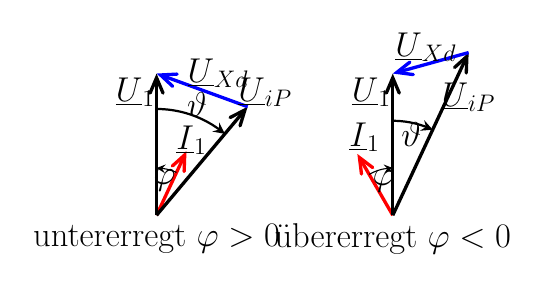
\begin{tikzpicture}[scale=.6, transform shape, font=\huge, >=angle 45]
	% UNTERERREGT
	\begin{scope}		
		\draw [very thick, red, ->] (0, 0) -- (65:1.5);
		\draw [very thick, ->] (0, 0) -- (0, 3);
		\draw [very thick, ->] (0, 0) -- (50:3);
		\draw [thick, ->, >=stealth] (0, 2.25) arc (90:50:2.25);
		\draw [very thick, blue, ->] (50:3) -- (0, 3);
		\draw [<-, >=stealth] (0, 1) arc (90:65:1);
		
		% BESCHRIFTUNGEN
		\draw (0,-0.5) node {untererregt $\varphi > 0$};
		
		\draw (70:2.5) node {$\vartheta$};
		\draw (-0.45, 2.6) node {$\underline U_1$};
		\draw (1.3, 3) node {$\underline U_\text{Xd}$};
		\draw (2.3, 2.6) node {$\underline U_\text{iP}$};
		\draw (65:1.75) node {$\underline I_1$};
		\draw (77:0.75) node{$\varphi$};
	\end{scope}
	
	% ÜBERERREGT
	\begin{scope}[shift={(5,0)}]
		\draw [very thick, red, ->] (0, 0) -- (120:1.5);
		\draw [very thick, ->] (0, 0) -- (0, 3);
		\draw [very thick, ->] (0, 0) -- (65:3.8);
		\draw [thick, ->, >=stealth] (0, 2) arc (90:65:2);
		\draw [very thick, blue, ->] (65:3.8) -- (0, 3);
		\draw [<-, >=stealth] (0, 1) arc (90:120:1);
		
		% BESCHRIFTUNGEN
		\draw (0,-0.5) node {übererregt $\varphi < 0$}; 
		
		\draw (77:1.75) node {$\vartheta$};
		\draw (-0.45, 2.6) node {$\underline U_1$};
		\draw (0.7, 3.55) node {$\underline U_\text{Xd}$};
		\draw (1.6, 2.5) node {$\underline U_\text{iP}$};
		\draw (110:1.75) node {$\underline I_1$};
		\draw (105:0.75) node{$\varphi$};
	\end{scope}
	
\end{tikzpicture}
\end{center}

\textbf{Generatorbetrieb:} $\vartheta > 0$ ($R_1 = 0$ VZS - Betrieb am starren Netz)
\begin{center}
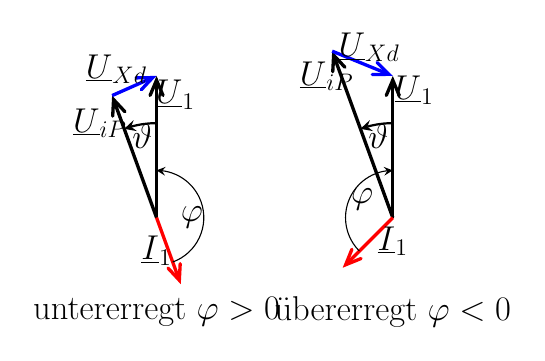
\begin{tikzpicture}[scale=.6, transform shape, font=\huge, >=angle 45]
	
	% UNTERERREGT
	\begin{scope}
		\draw [very thick, ->] (0, 0) -- (0, 3);
		\draw [very thick, ->] (0, 0) -- (110:2.75);
		\draw [very thick, red, ->] (0, 0) -- (290:1.5);
		\draw [thick, ->, >=stealth] (0, 2) arc (90:110:2);
		\draw [very thick, blue, ->] (110:2.75) -- (0, 3);
		\draw [->, >=stealth] (290:1) arc (-70:90:1);
		
		%BESCHRIFTUNGEN
		\draw (0,-2) node {untererregt $\varphi > 0$}; 
		
		\draw (100:1.75) node {$\vartheta$};
		\draw (0.4, 2.6) node {$\underline U_1$};
		\draw (-0.85, 3.15) node {$\underline U_\text{Xd}$};
		\draw (-1.2, 2.0) node {$\underline U_\text{iP}$};
		\draw (0, -0.7) node {$\underline I_1$};
		\draw (0:0.75) node{$\varphi$};
	\end{scope}
	
	% ÜBERERREGT
	\begin{scope}[shift={(5,0)}]
		\draw [very thick, ->] (0, 0) -- (0, 3);
		\draw [very thick, ->] (0, 0) -- (110:3.75);
		\draw [very thick, red, ->] (0, 0) -- (225:1.5);
		\draw [thick, ->, >=stealth] (0, 2) arc (90:110:2);
		\draw [very thick, blue, ->] (110:3.75) -- (0, 3);
		\draw [->, >=stealth] (225:1) arc (225:90:1);
	
		%BESCHRIFTUNGEN
		\draw (0,-2) node {übererregt $\varphi < 0$};
		
		\draw (100:1.75) node {$\vartheta$};
		\draw (0.45, 2.7) node {$\underline U_1$};
		\draw (-0.5, 3.6) node {$\underline U_\text{Xd}$};
		\draw (-1.4, 3) node {$\underline U_\text{iP}$};
		\draw (0, -0.5) node {$\underline I_1$};
		\draw (150:0.75) node{$\varphi$};
	\end{scope}
	
\end{tikzpicture}
\end{center}
\end{sectionbox}

\begin{sectionbox}
\subsection{Zeigerdiagramm}
\begin{center}
%!tikz editor 1.0
%!tikz source begin
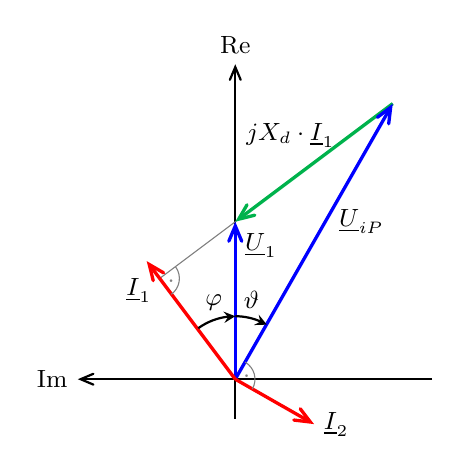
\begin{tikzpicture} [>=angle 45, font=\small]

% Koordinatensystem
\draw [->, thick] (2.5, 0) -- (-2, 0) node [left] {Im};
\draw [->, thick] (0, -0.5) -- (0, 4) node [above] {Re};

% Zeiger
\coordinate (U1) at (0,2);
\coordinate (Uip) at (2,3.5);
\coordinate (I1) at (-9/8,1.5);
\coordinate (I2) at (1,-0.57);
\coordinate (recht) at ($(0,0)!(Uip)!(I1)$);

\draw [black!50!white] (Uip) -- (recht);
\draw [->, very thick, green!70!blue] (Uip) -- (U1);
\draw [->, very thick, blue] (0, 0) -- (U1);
\draw [->, very thick, blue] (0, 0) -- (Uip);
\draw [->, very thick, red] (0, 0) -- (I1);
\draw [->, very thick, red] (0,0) -- (I2);

% Winkel
\draw [->, thick, >=stealth] (0, 0.8) arc (90:60:0.8);
\draw [<-, thick, >=stealth] (0, 0.8) arc (90:126:0.8);
\draw [black!50!white] (recht) ++(36:0.25) arc (36:-54:0.25);
\draw (recht) ++(-15:0.15) node [black!50!white] {.};
\draw [black!50!white] (0,0) ++(60:0.25) arc (60:-30:0.25);
\draw (0,0) ++(15:0.15) node [black!50!white] {.};

% Beschriftung
\draw (I1) ++(-0.1, -0.1) node [below] {$\underline I_1$};
\draw (U1) ++(0, -0.3) node [right] {$\underline U_1$};
\draw (U1) ++(1.6, 0) node {$\underline U_\text{iP}$};
\draw (Uip) ++(-1.3,-0.4) node {$jX_d\cdot\underline I_1$};
\node at (I2) [right] {$\underline I_2$};

\draw (75:0.8) node [above] {$\vartheta$};
\draw (110:0.8) node [above] {$\varphi$};
\end{tikzpicture}
%!tikz source end

\end{center}
\end{sectionbox}

\begin{sectionbox}
\subsection{Stromortskurve}
\begin{align*}
\underline{I}_1 &= \underline{I}_{K0} - \underline I_{K\textrm{III}}\\
\underline I_{K\textrm{III}} &= \frac{U_\text{iP}}{U_1}\cdot \underline{I}_{K0}\cdot e^{j\vartheta}\\
\underline{I}_{K0} &= -\frac{U_1}{Z_1}\cdot j\, e^{j\varphi_{Z1}}
\end{align*}
\begin{cookbox}{Stromortskurve}
\item $\underline{U}_1$ auf reelle Achse legen
\item Richtung von $\underline{U}_\text{iP}$ einzeichnen
\item $\underline{I}_{K0}$ einzeichnen\\
bei $R_1 = 0:\ \underline{I}_{K0}$ eilt $\underline{U}_1$ um $\ang{90}$ nach
\item konstante Erregung: Kreis um Spitze von $\underline{I}_{K0}$ mit Radius $I_{K\textrm{III}}$
\item Richtungen von $\underline{I}_{K\textrm{III}}$ und $\underline{I}_1$ festgelegt durch $\varphi$ bzw. $\vartheta$
\item bei $R_1 = 0$: Verlängerung von $\underline{U}_\text{iP} \perp \underline{I}_{K\textrm{III}}$
\end{cookbox}
\begin{center}
%!tikz editor 1.0
%!tikz source begin
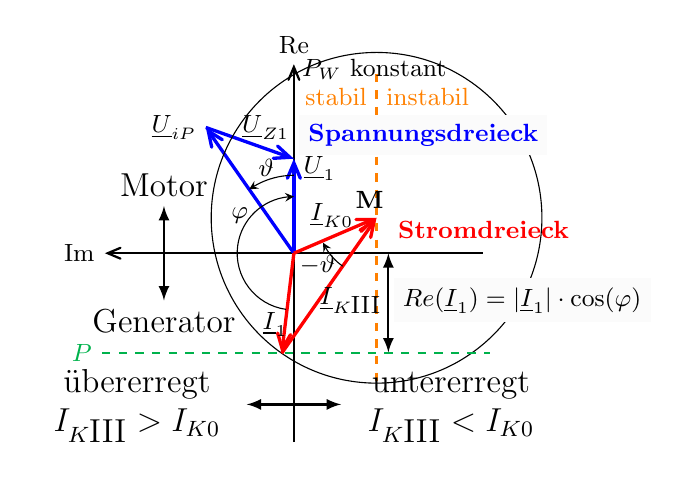
\begin{tikzpicture} [scale=.6, >=angle 45, font=\small]

% Koordinatensystem
\draw [->, thick] (4, 0) -- (-4, 0) node [left] {Im};
\draw [->, thick] (0, -4) -- (0, 4) node [above] {Re};

% Zeiger
\draw [->, very thick, blue] (0, 0) -- (0, 2);
\draw [->, very thick, blue] (0, 0) -- (125:3.25);
\draw [->, very thick, blue] (125:3.25) -- (0, 2);

\draw (1.75, 0.75) circle (3.5);

\draw [->, very thick, red] (0, 0) -- (1.75, 0.75);
\draw [<-, very thick, red] (1.75, 0.75) -- ++(235:3.5);
\draw [<-, very thick, red] (1.75, 0.75) ++(235:3.5) -- (0, 0); 

\draw [->, >=stealth] (0, 1.65) arc (90:125:1.65);
\draw [->, >=stealth] (262:1.2) arc (262:90:1.2);
\draw [->, >=stealth] (1.75, 0.75) ++(235:1.25) arc (235:205:1.25);

\draw [dashed, thick, green!70!blue] (1.75, 0.75) ++(235:3.5) +(-3.8,0) node [left] {$P$} -- +(4.4, 0) ;

\draw [dashed, thick, red!50!yellow] (1.75, 3.8) -- (1.75, -2.7); 

% Beschriftungspfeile
\draw [<->, >=latex, thick] (2,0) -- (2, -2.1);
\draw [<->, >=latex, thick] (-2.75, 1) -- (-2.75, -1);
\draw [<->, >=latex, thick] (-1, -3.2) -- (1, -3.2);

% Beschriftung
\draw (1.6, 0.75) node [above] {\textbf M};
\draw (-1, -3.2) node [left, font=\large] {\begin{tabular}{c} übererregt \\ $I_{K\textrm{III}} > I_{K0}$ \end{tabular}};
\draw (1, -3.2) node [right, font=\large] {\begin{tabular}{c} untererregt\\ $I_{K\textrm{III}} < I_{K0}$ \end{tabular}};
\draw (-2.75, 1) node [above, font=\large] {Motor};
\draw (-2.75, -1) node [below, font=\large] {Generator};
\draw (2.1, -1) node [right, fill=gray!3] {$\text{Re}(\underline I_1) = |\underline I_1| \cdot \cos(\varphi)$};

\draw (0, 1.8) node [right] {$\underline U_1$};
\draw (-0.6, 2.2) node [above] {$\underline U_{Z1}$};
\draw (125:3.25) node [left] {$\underline U_\text{iP}$};

\draw (0.8, 0.8) node {$\underline I_{K0}$};
\draw (1.2, -1) node {$\underline I_{K\textrm{III}}$};
\draw (-0.4, -1.5) node {$\underline I_1$};

\draw (108:1.9) node {$\vartheta$};
\draw (145:1.4) node {$\varphi$};
\draw (0.5, -0.25) node {$-\vartheta$};

\draw (0.1, 2.5) node [right, blue, fill=gray!3] {\textbf{Spannungsdreieck}};
\draw (2, 0.5) node [right, red] {\textbf{Stromdreieck}};
\draw (1.7, 3.9) node {$P_W$ konstant};
\draw (1.75, 3.3) node [left, red!50!yellow] {stabil};
\draw (1.75, 3.3) node [right, red!50!yellow] {instabil}; 

\end{tikzpicture}
%!tikz source end

\end{center}
\end{sectionbox}

\begin{sectionbox}
\subsection{dq-Darstellung}
\begin{cookbox}{Zeigerdiagramm}
\item $\underline{U}_1$ auf reelle Achse legen
\item $\underline{I}_1$ einzeichnen
\item Richtung von $U_\text{iP}$ legt $d$ und $q$ Achse fest\\
($\vartheta =$ unbekannt $\Rightarrow$ weiter bei Trick)
\item Zerlegung von $\underline{I}_1$ in $\underline{I}_d$ und $\underline{I}_q$
\item Spannungsabfall an $X_d = \abs{X_d\cdot I_d}$
\item Spannungsabfall an $X_q = \abs{X_q\cdot I_q}$
\item $\underline{U}_\text{iP} = \underline{U}_1 - jX_d\cdot\underline{I}_d - jX_q\cdot\underline{I}_q$
\end{cookbox}
\begin{cookbox}{Trick}
\item $\vartheta = \arg(\underline{U}_1 - jX_q\cdot\underline{I}_1) \Rightarrow$ Richtungsgerade von $U_\text{iP} (||jX_d \underline I_d)$
\item $\underline{U}_\text{iP} =$ Senkrechte von $\underline{U}_1 - jX_d\cdot\underline{I}_d$ auf Richtungsgerade
\end{cookbox}

\subsubsection{Systemgleichungen}
\begin{align*}
U_d &= R_1\cdot I_d - \omega_1 L_q\cdot I_q\\
U_q &= R_1\cdot I_q + \omega_1 L_d\cdot I_d + \sqrt{2}\cdot U_\text{iP}\\
U_\text{iP} &= \sqrt{2}\cdot \omega_1 M_{21}\cdot I_2\\
U_2 &= R_2\cdot I_2\\
M_i &= 3\cdot p\cdot M_{21}\cdot I_2\cdot I_q
\end{align*}

\subsubsection{Zeigerdiagramm}
\begin{center}
%!tikz editor 1.0
%!tikz source begin
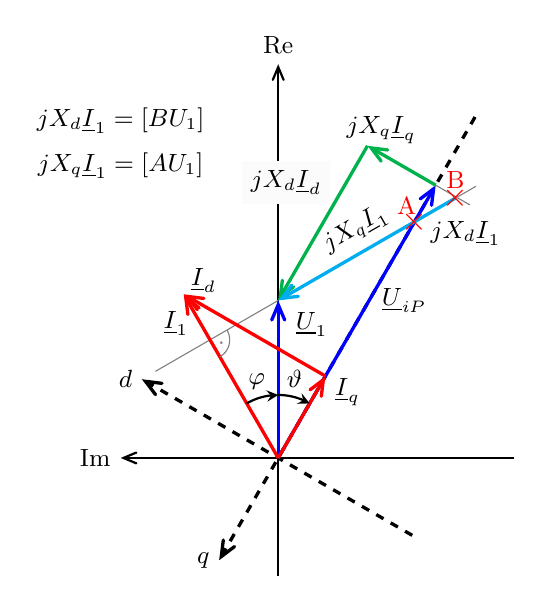
\begin{tikzpicture} [>=angle 45, font=\small]

% Koordinatensystem
\draw [->, thick] (3, 0) -- (-2, 0) node [left] {Im};
\draw [->, thick] (0, -1.5) -- (0, 5) node [above] {Re};

% Zeiger
\coordinate (U1) at (0,2);
\coordinate (Uip) at (60:4);
\coordinate (Iq) at (60:1.2);
\coordinate (I1) at (120:2.4);
\coordinate (q) at (240:1.5);
\coordinate (d) at (150:2);
\coordinate (recht) at ($(0,0)!(U1)!(I1)$);

\draw [->, very thick, dashed] (Uip) +(60:1) -- (q);
\draw [<-, very thick, dashed] (d) -- ++(-30:4);

\draw [black!50!white] (Uip) -- ++(-30:0.5);
\draw [black!50!white] (U1) -- +(210:1.8) ++(30:2.6) -- ++(30:0.3);

\draw [->, very thick, blue] (0, 0) -- (U1);
\draw [name path=Uline, ->, very thick, blue] (0, 0) -- (Uip);
\draw [->, very thick, red] (0, 0) -- (I1);
\draw [->, very thick, red] (0, 0) -- (Iq);
\draw [->, very thick, red] (Iq) -- (I1);

\draw [->, very thick, green!70!blue] (Uip) -- ++(150:1);
\draw [->, very thick, green!70!blue] (Uip) ++(150:1) -- (U1);
\draw [name path=Xline, <-, very thick, cyan] (U1) -- ++(30:2.6) node [midway, above, sloped, black] {$jX_q\underline I_1$};

\path [name intersections={of=Uline and Xline, by=A}];

% Winkel
\draw [->, thick, >=stealth] (0, 0.8) arc (90:60:0.8);
\draw [<-, thick, >=stealth] (0, 0.8) arc (90:120:0.8);
\draw [>=stealth, black!50!white] (recht) ++(30:0.25) arc (30:-60:0.25);
\draw (recht) ++(-15:0.15) node [black!50!white] {.};

% Beschriftung
\draw (d) node [left] {$d$};
\draw (q) node [left] {$q$};
\draw (Iq) ++(0, -0.2) node [right] {$\underline I_q$};
\draw (I1) ++(-0.1, -0.1) node [below] {$\underline I_1$};
\draw (I1) ++(0.25, -0.1) node [above] {$\underline I_d$};
\draw (U1) ++(0.1, -0.3) node [right] {$\underline U_1$};
\draw (U1) ++(1.6, 0) node {$\underline U_\text{iP}$};
\draw (Uip) ++(150:.8) node [above] {$jX_q \underline I_q$};
\draw (0.1, 3.5) node [fill=gray!3] {$jX_d\underline I_d$};
\draw (U1) ++(25:2) node [right] {$jX_d\underline I_1$};

\node at (A) [red, font=\large] {$\times$};
\draw [red] (A) ++(-0.1,0.2) node {A};
\draw (U1) ++(30:2.6) node [red, font=\large] {$\times$};
\draw (U1) ++(30:2.6) node [red, above] {B};

\node at (-2,4) [above] {$jX_d\underline I_1 = [BU_1]$};
\node at (-2,4) [below] {$jX_q\underline I_1 = [AU_1]$};

\draw (75:0.8) node [above] {$\vartheta$};
\draw (110:0.8) node [above] {$\varphi$};
\end{tikzpicture}
%!tikz source end

\end{center}
\end{sectionbox}

\begin{sectionbox}
\subsection{Schenkelpolläufer}
\subsubsection{Drehmoment ($R_1 = 0$)}
\begin{emphbox}
\[M_i' = -\frac{m_1\cdot p}{\omega_1} U_1\left[\frac{U_\text{iP}}{X_d}\sin(\vartheta) + \frac{U_1}{2}\left(\frac{1}{X_q} - \frac{1}{X_d}\right)\sin(2\vartheta)\right]\]
\end{emphbox}
\textbf{Reluktanzmoment (Reaktionsmoment):}
\begin{align*}
M_r = -\frac{m_1\cdot p}{\omega_1}\cdot\frac{{U_1}^2}{2}\left(\frac{1}{X_q} - \frac{1}{X_d}\right)\sin(2\vartheta)
\end{align*}
Vollpolläufer entwickeln kein Reluktanzmoment wegen $L_d = L_q$.\\
Maximales Reluktanzmoment bei $\abs{\vartheta} = \SI{45}{\degree}$.

\subsubsection{Systemgleichungen}
\begin{align*}
\underline{U}_1 &= \underline{U}_d + \underline{U}_q + \underline{U}_\text{iP}\\
&= jX_d\cdot\underline{I}_d + jX_q\cdot\underline{I}_q + \underline{U}_\text{iP}\\
\underline{I}_1 &= \underline{I}_d + \underline{I}_q
\end{align*}
\end{sectionbox}

\section{Asynchronmaschine}
\begin{sectionbox}
\subsection{Größen}
\begin{tablebox}{p{4,5cm}cc}
Übersetzungsverhältnis & $\ddot{u}$ & $\unitof{\si{1}}$\\
Schlupf & $s$ & $\unitof{\si{1}}$\\
Kippschlupf & $s_K$ & $\unitof{\si{1}}$\\
Kippmoment & $M_K$ & $\unitof{\si{\newtonmeter}}$\\
\cmrule
Bezogener Statorwiderstand & $\rho_1$ & $\unitof{\si{1}}$\\
Bezogener Rotorwiderstand & $\rho_2$ & $\unitof{\si{1}}$\\
Hilfsgröße & $\Delta\rho_1$ & $\unitof{\si{1}}$\\
\cmrule
Rotor-Statorwärmeverluste & $P_\text{Cu}$ & $\unitof{\si{\watt}}$\\
Magnetisierungsstrom & $\underline{I}_{1\mu}$ & $\unitof{\si{\ampere}}$\\
Rotor-Vorwiderstand & $R_{2V}$ & $\unitof{\si{\ohm}}$\\
\end{tablebox}
\end{sectionbox}

\begin{sectionbox}
\subsection{ESB}
\begin{center}
\begin{circuitikz}[scale=.75, transform shape, font=\large]
\draw [american currents]
	(0,2)
	to [short, i=$\underline{I}_1$, o-](.5, 2)
	to [R=\mbox{$R_\text{Fe}=\frac{3\cdot{U_1}^2}{P_\text{Fe}}$}, *-*] (.5,0)
	(.5,2)
	to [R=\mbox{$R_1(=0)$}](2,2) 
	to [L=$j\omega_1L_{1\sigma}$](4,2)
	to [L=$j\omega_1L_{1h}$, i=$\underline{I}_{1\mu}$, v>=$\underline{U}_{1i}$, *-*] (4,0)
	(4,2)
	to [L=$j\omega_1L_{2\sigma}'$](6,2)
	to [R=$R_{2,\text{ges}}'$, i<=$\underline{I}_2'$](8,2)
	to [R, l_=$R_{2,\text{ges}}'\cdot\frac{1-s}{s}$] (8,0) 
	to [short, -o]	(0,0);
\draw[->, >=latex] (0,1.8) -- (0,0.2) node [pos=0.5, left] {$\underline U_1$};
\end{circuitikz}


\end{center}

\subsubsection{Übersetzungsverhältnis}
Bei Schleifring-ASM gilt: $\quad M_{21} = M_{12} = M$

\begin{symbolbox}
\begin{center}
$\ddot{u} = \dfrac{L_{1h}}{M} = \sqrt{\frac{m_1}{m_2}}\cdot\frac{w_1\xi_1}{w_2\xi_2}\cdot\frac{1}{\xi_\text{Schr}} = \sqrt{\frac{m_1}{m_2}}\cdot\frac{w_{1,\text{eff}}}{w_{2,\text{eff}}}\cdot\frac{1}{\xi_\text{Schr}}$
\end{center}
\end{symbolbox}
\begin{tabularx}{\columnwidth}{CC}
$R_{2,\text{ges}}' = \ddot{u}^2\cdot R_{2,\text{ges}}$ & $R_{2,\text{ges}}' = R_2' + R_{2V}'$\\
$\underline U_2 = \frac{1}{\ddot{u}}\cdot\underline U_{1i}$ &  $L_{2\sigma}' = \ddot{u}^2\cdot (L_{2\sigma} + L_{2\text{Schr}})$\\
$\underline{I}_2' = \frac{1}{\ddot{u}}\cdot\underline{I}_2$ &
\end{tabularx}

\subsection{Systemgleichungen}
\begin{align*}
\vec{u}_1 &= R_1\cdot\vec{i}_1 + \frac{\partial\vec\Psi_1}{\partial t}, & \vec\Psi_1 &= L_1\cdot\vec i_1 + M\cdot\vec i_2\cdot e^{jp\vartheta_m}\\
0 &= R_{2,\text{ges}}\cdot\vec{i}_2 + \frac{\partial\vec\Psi_2}{\partial t}, & \vec\Psi_2 &= L_2\cdot\vec i_2 + M\cdot\vec i_1\cdot e^{-jp\vartheta_m}\\
J\frac{\diff\omega}{\diff t} &= M_i - M_R - M_L
\end{align*}
\end{sectionbox}

\begin{sectionbox}
\subsection{Wichtige Größen}
\subsubsection{Schlupf}
\begin{emphbox}
$s = \frac{n_\text{syn} - n}{n_\text{syn}} = \frac{\omega_\text{syn} - \omega_m}{\omega_\text{syn}} = \frac{\omega_1 - p\cdot\omega_m}{\omega_1} = \frac{\omega_2}{\omega_1}$
\end{emphbox}
\begin{tabularx}{\columnwidth}{CCC}
Gegenstrombremse & Motor & Generator\\
$s > 1$ & $1 > s > 0$ & $s < 0$
\end{tabularx}

\subsubsection{Drehzahl}
\begin{tabularx}{\columnwidth}{CC}
synchrone Drehzahl & Nenndrehzahl\\
$n_\text{syn} = \frac{f}{p}$ & $n_N = n_s (1-s_N)$
\end{tabularx}

\subsubsection{Leistung}
\begin{align*}
\underline{S}_1 &= m_1\cdot \underline{U}_1\cdot\underline{I}_1^*\\
P_1 &= S_1 \cdot\cos{(\varphi)} = m_1\cdot U_1\cdot I_1\cdot\cos{(\varphi)}\\
P_\text{Netz} &= m_1\cdot U_1\cdot I_1\cdot\cos{(\varphi_N)} = P_1 + P_\text{Fe}\\
P_\delta &= 2\pi\cdot n_\text{syn}\cdot M_i = P_1 - P_{\text{Cu}1} - P_\text{Fe}\\
P_{mi} &= (1-s)P_\delta = P_\delta - P_{\text{Cu}2} - P_{2V} = \omega_m\cdot M_i\\
P_m &= 2\pi\cdot n\cdot (M_i - M_R) = \omega_m\cdot (M_i - M_R) = P_{mi} - P_R\\
P_{\text{Cu}2} &= s\cdot P_\delta = m_2\cdot R_2\cdot {I_2}^2\\
\end{align*}

\subsubsection{Phase}
\begin{emphbox}
ASM immer induktiv $\Rightarrow \varphi > 0$
\end{emphbox}
\begin{align*}
\varphi &= \varphi_{1Z}-\varphi_{1N}\\
\varphi &= \begin{cases}
\arctan(\frac{b}{a}) & \text{für } a > 0\\
\arctan(\frac{b}{a})+\pi & \text{für } a < 0, b\geq 0\\
\arctan(\frac{b}{a})-\pi & \text{für } a < 0, b<0
\end{cases}
\end{align*}
\end{sectionbox}

\begin{sectionbox}
\subsubsection{Weitere Parameter}
\begin{tabularx}{\columnwidth}{CC}
$L_{1\sigma} = \sigma_1\cdot L_{1h}$ & $L_1 = L_{1h} + L_{1\sigma}$\\
$L_{2\sigma}' = \sigma_2\cdot L_{1h}$ & $L_2' = L_{1h}\cdot (1+\sigma_2)$\\
\multicolumn{2}{c}{$L_\sigma = \sigma\cdot L_1 = L_{1\sigma} + \frac{\xi_\text{Schr}}{1 + \sigma_2}L_{2\sigma}'$}\\
$\rho_1 = \frac{R_1}{\omega_1 L_1}$ & $\rho_2 = \frac{R_{2,\text{ges}}}{\omega_1 L_2} = \frac{R_{2,\text{ges}}'}{\omega_1 L_2'}$\\
\multicolumn{2}{c}{$\Delta \rho_1 = \sqrt{1+\left( \frac{\rho_1}{\sigma}\right)^2}\cdot\sqrt{1+{\rho_1}^2}$}\\
\multicolumn{2}{c}{$\sigma = 1 - \frac{1}{(1 + \sigma_1)\cdot(1 + \sigma_2)} = 1 - \frac{M^2}{L_1 L_2}$}
\end{tabularx}
\end{sectionbox}

\begin{sectionbox}
\subsection{Statorstrom}
\begin{emphbox}
\[\underline{I}_1 = \frac{\underline{U}_1}{\omega_1 L_1} \cdot \frac{\rho_2 +js}{\rho_1\cdot\rho_2 -\sigma\cdot s+j(\rho_2 +s\cdot \rho_1)}\]
\end{emphbox}
Anlaufstrom:\\
$I_{1A} = |\underline{I}_1|(s=1) = \frac{U_1}{\omega_1 L_\sigma}\sqrt{\frac{1+{\rho_2}^2}{\left(1-\frac{\rho_1\cdot\rho_2}{\sigma}\right)^2 +\left(\frac{\rho_1+\rho_2}{\sigma}\right)^2}}$\\
Ideeller Kurzschlussstrom:\\
$I_{1Ki} = |\underline{I}_1|(s\rightarrow\pm\infty) = \frac{U_1}{\omega_1 L_\sigma}\cdot \frac{1}{\sqrt{1+\left( \frac{\rho_1}{\sigma}\right)^2}}$\\
Leerlaufstrom:\\$I_{10} = |\underline{I}_1|(s=0) = \frac{U_1}{\omega_1 L_1}\cdot \frac{1}{\sqrt{1+{\rho_1}^2}}$

\subsubsection{Magnetisierungsstrom}
\[\underline I_\mu = \frac{\rho_2 + j\cdot s\cdot(\sigma - \sigma_1\cdot(1-\sigma))}{\rho_1\cdot\rho_2 - \sigma\cdot s + j\cdot(\rho_2 + s\cdot\rho_1)}\cdot\frac{\underline U_1}{\omega_1 L_1}\]
\end{sectionbox}

\begin{sectionbox}
\subsection{Zeigerdiagramm}
\begin{cookbox}{Zeigerdiagramm}
\item $\underline{U}_1$ auf reelle Achse legen und $\underline{I}_1$ einzeichnen
\item $R_1\underline{I}_1$ (gleiche Phasenlage wie $\underline{I}_1$)\\
$j\omega_1 L_{1\sigma}\underline{I}_1$ (eilt $\underline{I}_1$ um $\ang{90}$ voraus)
\item $\underline{U}_{1i} = \underline{U}_1 - R_1\underline{I}_1 - j\omega_1 L_{1\sigma}\underline{I}_1$
\item $\underline{I}_{1\mu} = \frac{\underline{U}_{1i}}{j\omega_1 L_{1h}}$ (eilt $\underline{U}_{1i}$ um $\ang{90}$ nach)
\item $\underline{I}_2' = \underline{I}_{1\mu} - \underline{I}_1$
\item $R_{2,\text{ges}}'\underline{I}_2'$ (parallel zu $\underline{I}_2'$)
\item $j\omega_1 L_{2\sigma}'\underline{I}_2'$ (eilt $\underline{I}_2'$ um $\ang{90}$ voraus)
\item $R_{2,\text{ges}}'\cdot\frac{1-s}{s}\cdot\underline{I}_2' = -\underline{U}_{1i} - R_{2,\text{ges}}'\,\underline{I}_2' - j\omega_1 L_{2\sigma}'\underline{I}_2'$
\end{cookbox}
\begin{center}
%!tikz editor 1.0
%!tikz source begin
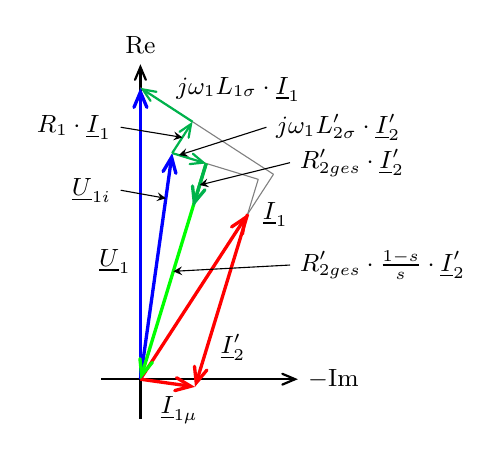
\begin{tikzpicture} [>=angle 45, font=\small]

% Koordinatensystem
\draw [->, thick] (-0.5, 0) -- (2, 0) node [right] {$-$Im};
\draw [->, thick] (0, -0.5) -- (0, 4) node [above] {Re};

% Koordinaten
\coordinate (U1) at (0,3.7);
\coordinate (I1) at (57:2.5);
\coordinate (Ui1) at (82:2.9);
\coordinate (I1u) at (-8:0.7);

\coordinate (P1) at ($(0,0)!(U1)!(I1)$);
\coordinate (P2) at ($(I1u)!(Ui1)!(I1)$);
\coordinate (P3) at ($(P2)!(0,0)!(I1)$);
\coordinate (P4) at ($(U1)!(Ui1)!(P1)$);
\coordinate (P5) at ($(Ui1)!(0,0)!(P2)$);

\draw [black!50!white] (0,0) -- (P1);
\draw [black!50!white] (P1) -- (U1);
\draw [black!50!white] (Ui1) -- (P2);
\draw [black!50!white] (I1) -- (P2);

\draw [->, very thick, blue] (0, 0) -- (U1);
\draw [->, very thick, red] (0, 0) -- (I1);
\draw [->, very thick, blue] (0, 0) -- (Ui1);
\draw [->, very thick, red] (0, 0) -- (I1u);
\draw [->, very thick, red] (I1) -- (I1u);

\draw [->, thick, green!70!blue] (Ui1) -- (P4);
\draw [->, thick, green!70!blue] (P4) -- (U1);
\draw [->, thick, green!70!blue] (Ui1) -- (P5);
\draw [->, very thick, green] (P5) -- (0, 0);
\draw [->, very thick, green!70!blue] (P5) -- ($(P5)!0.2!(0,0)$);

% Beschriftungspfeile
\draw [->, >=stealth] (-0.25, 2.4) -- ($(0,0)!0.8!(Ui1)$);
\draw [->, >=stealth] (-0.25, 3.2) -- ($(P4)!0.5!(Ui1)$);
\draw [->, >=stealth] (1.6, 3.2) -- ($(Ui1)!0.2!(P5)$);
\draw [->, >=stealth] (1.9, 2.75) -- ($(P5)!0.1!(0,0)$);
\draw [->, >=stealth] (1.9, 1.45) -- ($(P5)!0.5!(0,0)$);

% Beschriftung
\node [left] at (0, 1.5) {$\underline U_1$};
\node [right=2] at (I1) {$\underline I_1$};
\draw (I1u) +(-0.2,0) node [below] {$\underline I_{1\mu}$};
\draw (I1u) +(0.2,0.5) node [right] {$\underline I_{2}'$};
\node [left] at (-0.25, 2.4) {$\underline U_{1i}$};
\draw ($(P4)!0.5!(U1)$) +(0,0.2) node [right] {$j\omega_1 L_{1\sigma} \cdot\underline I_1$};
\draw (-0.25, 3.2) node [left] {$R_1\cdot \underline I_1$};
\draw (1.6, 3.2) node [right] {$j\omega_1 L_{2\sigma}' \cdot \underline I_2'$};
\draw (1.9, 2.75) node [right] {$R_{2\text{ges}}'\cdot\underline I_2'$};
\draw (1.9, 1.45) node [right] {$R_{2\text{ges}}'\cdot \frac{1-s}{s}\cdot\underline I_2'$};
\end{tikzpicture}
%!tikz source end

\end{center}
\end{sectionbox}

\begin{sectionbox}
\subsection{Stromortskurve}
\begin{symbolbox}
  bei $R_1 = 0\qquad\qquad\qquad\tan(\mu) = s_K$
\end{symbolbox}
\begin{cookbox}{Stromortskurve $R_1 = 0\wedge R_\text{Fe} = 0$}
\item $\underline{U}_1$ auf reelle Achse legen $\Rightarrow\varphi_{1U} = 0$
\item $R_1 = 0\Rightarrow \underline I_{10}$ und $\underline I_{1Ki}$ haben keinen Realteil
\item Kreismittelpunkt auf Im-Achse zwischen $\underline{I}_{1Ki}$ und $\underline{I}_{10}$
\item $\mu$ zwischen $P_0$ und $P_A$
\end{cookbox}
%!tikz editor 1.0
%!tikz source begin
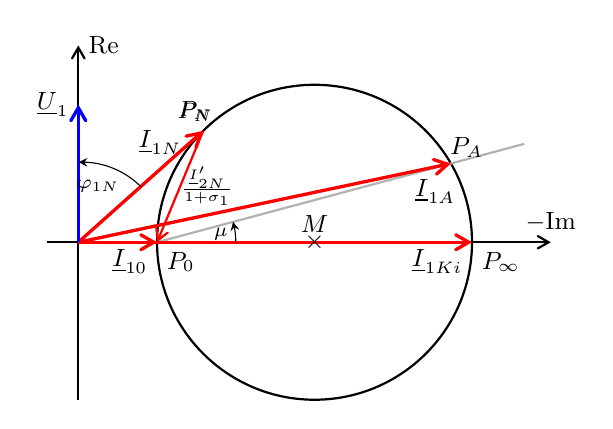
\begin{tikzpicture}[>=angle 60, font=\small]

% Koordinatensystem
\draw [->, thick] (-.4, 0) -- (6, 0) node [above] {$-$Im};
\draw [->, thick] (0, -2) -- (0, 2.5) node [right] {Re};

% Kreis
\coordinate (M) at (3, 0);
\draw [thick] (M) circle (2);

% Vektoren
\coordinate (U1) at (0, 1.75);
\coordinate (Iki1) at ($(M)+(2,0)$);
\coordinate (I01) at ($(M)+(-2,0)$);
\coordinate (Ia1) at ($(M)+(30:2)$);
\coordinate (In1) at ($(M)+(135:2)$);

\draw [thick, black!30!white] (I01) -- ($(I01)!1.25!(Ia1)$);
\draw [->, very thick, red] (0, 0) -- (Iki1);
\draw [->, very thick, red] (0, 0) -- (Ia1);
\draw [->, very thick, red] (0, 0) -- (In1);
\draw [->, very thick, red] (0, 0) -- (I01);
\draw [->, very thick, blue] (0, 0) -- (U1);
\draw [->, thick, red] (In1) -- (I01);

% Winkel
\draw [->, >=stealth] (I01)+(1,0) arc (0:15:1);
\coordinate (phi) at ($(0,0)!0.5!(In1)$);
\draw [->, >=stealth] (phi) let \p1 = (phi) in arc (45:92:({veclen(\x1,\y1)}););
%\draw [->, >=stealth] (0,0)+(0.5,0.5) arc (45:90:0.707);

% Beschriftung
\node at (M) [above] {$M$};
\node at (M) {$\times$};
\node at (U1) [left] {$\underline U_1$};
\draw (In1) +(-0.55, -0.15) node {$\underline I_{1N}$}
			+(-0.1, 0.25) node {$P_N$};
\draw (Ia1) +(-0.2, -0.35) node {$\underline I_{1A}$}
			+(0.2, 0.2) node {$P_A$};
\draw (Iki1)+(0, -0.25) node [left] {$\underline I_{1Ki}$}
			+(0, -0.25) node [right] {$P_\infty$};
\draw (I01)+(0, -0.25) node [left] {$\underline I_{10}$}
			+(0, -0.25) node [right] {$P_0$};
\draw (In1) +(0.05, -0.7) [font=\scriptsize] node {$\frac{\underline I_{2N}'}{1+\sigma_1}$}
			+(-0.1, 0.25) node {$P_N$};
\draw (I01)+(0.6,0.1) [right, font=\scriptsize] node {$\mu$};
\draw (phi)+(-0.15,0) [left, font=\scriptsize] node {$\varphi_{1N}$};
			
\end{tikzpicture}
%!tikz source end

\end{sectionbox}

\begin{sectionbox}
\subsubsection{Schlupfgerade}
\begin{cookbox}{Schlupfgerade $R_1 = 0\wedge R_\text{Fe}\neq 0$}
\item (Bei $R_\text{Fe} = 0$) Mittelpunkt $M$ auf -Im Achse
\item Schlupfgerade an beliebiger Stelle einzeichnen
\item gesuchtes $s$ aus Längenverhältnis zu bekanntem Schlupf bestimmen
\end{cookbox}
%!tikz editor 1.0
%!tikz source begin
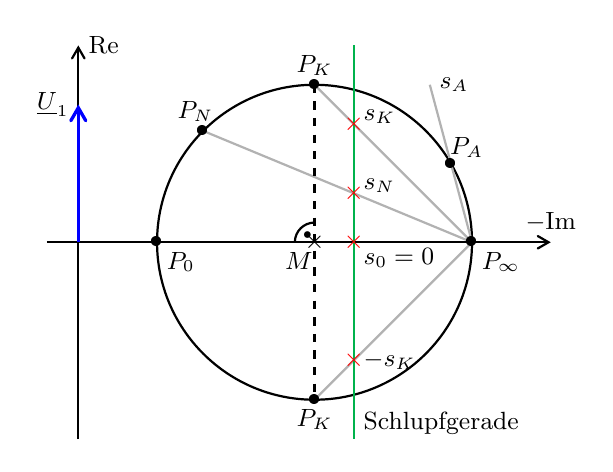
\begin{tikzpicture}[>=angle 60, font=\small]

% Koordinatensystem
\draw [->, thick] (-.4, 0) -- (6, 0) node [above] {$-$Im};
\draw [->, thick] (0, -2.5) -- (0, 2.5) node [right] {Re};

% Kreis
\coordinate (M) at (3, 0);
\draw [thick] (M) circle (2);

% Vektoren
\coordinate (U1) at (0, 1.75);
\coordinate (Iki1) at ($(M)+(2,0)$);
\coordinate (I01) at ($(M)+(-2,0)$);
\coordinate (Ia1) at ($(M)+(30:2)$);
\coordinate (In1) at ($(M)+(135:2)$);
\coordinate (Pko) at ($(M)+(0,2)$);
\coordinate (Pku) at ($(M)+(0,-2)$);
\coordinate (sa) at ($(Iki1)!2!(Ia1)$);
\coordinate (s0) at ($(M)+(0.5, 0)$);

\draw [->, very thick, blue] (0, 0) -- (U1);
\draw [name path=pnline, thick, black!30!white] (Iki1) -- (In1);
\draw [name path=pkoline, thick, black!30!white] (Iki1) -- (Pko);
\draw [name path=pkuline, thick, black!30!white] (Iki1) -- (Pku);
\draw [name path=paline, thick, black!30!white] (Iki1) -- (sa);

\draw [name path=sline, thick, green!70!blue]  (s0) +(0, 2.5) -- +(0, -2.5);

\path [name intersections={of=sline and pkoline, by=sko}];
\path [name intersections={of=sline and pkuline, by=sku}];
\path [name intersections={of=sline and pnline, by=sn}];

\draw [thick, dashed] (Pko) -- (Pku);
\draw [thick] (M) ++(0, 0.25) arc (90:180:0.25);
\draw (M) ++(135:0.125) node [font=\tiny] {$\bullet$};

% Beschriftung
\node at (M) {$\times$};
\node at (U1) [left] {$\underline U_1$};
\draw (M) +(-0.2,0) node [below] {$M$};
\draw (In1) +(-0.1, 0.25) node {$P_N$}
			+(0,0) node {\textbullet};
\draw (Ia1) +(0.2, 0.2) node {$P_A$}
			+(0,0) node {\textbullet};
\draw (Iki1)+(0, -0.25) node [right] {$P_\infty$}
			+(0,0) node {\textbullet};
\draw (I01)+(0, -0.25) node [right] {$P_0$}
			+(0,0) node {\textbullet};
\draw (Pko) node [above] {$P_K$}
			+(0,0) node {\textbullet};
\draw (Pku) node [below] {$P_K$}
			+(0,0) node {\textbullet};
\draw (s0) node[red] {$\times$}
			+(0,-0.2) node [right] {$s_0 = 0$};
\draw (sko) node[red] {$\times$}
			+(0,0.1) node [right] {$s_K$};
\draw (sku) node[red] {$\times$}
			+(0,0) node [right] {$-s_K$};
\draw (sn) node[red] {$\times$}
			+(0,0.1) node [right] {$s_N$};
\draw (sa) node [right] {$s_A$};
\draw (s0) +(0,-2.3) node [right] {Schlupfgerade}; 		

\end{tikzpicture}
%!tikz source end


\subsubsection{Maßstab}
\begin{symbolbox}
\begin{tabular}{p{2.8cm}cc}
Strommaßstab & $m_I$ & $\unitof{\si{\ampere\per\centi\meter}}$\\
Leistungsmaßstab & $m_P = m_1\cdot U_1\cdot m_I$ & $\unitof{\si{\watt\per\centi\meter}}$\\
Drehmomentmaßstab & $m_M = \frac{m_P}{2\pi\cdot n_\text{syn}}$ & $\unitof{\si{\newtonmeter\per\centi\meter}}$
\end{tabular}
\end{symbolbox}
\end{sectionbox}

\begin{sectionbox}
\subsubsection{Ablesbare Werte}
\begin{emphbox}
  $R_1\neq 0\wedge R_\text{Fe}\neq 0$
\end{emphbox}
\begin{tabular}{p{4cm}l}
Aufgenommene elektrische Leistung & $P_1 = \overline{PD}\cdot m_P$\\
Eisenverluste Stator & $P_\text{Fe} = \overline{CD}\cdot m_P$\\
Kupferverluste Stator & $P_{\text{Cu}1} = \overline{BC}\cdot m_P$\\
Kupferverluste Rotor & $P_{\text{Cu}2} = \overline{AB}\cdot m_P$\\
Abgegebene mechanische Leistung & $P_m = \overline{PA}\cdot m_P$\\
Inneres Drehmoment & $M_i = \overline{PB}\cdot m_M$
\end{tabular}
\begin{symbolbox}
  Definition Punkt D: Orthogonale Projektion von $P$ auf Im-Achse\\
  \begin{tabularx}{\columnwidth}{lX}
  $R_1 = 0$ & $B = C$ und $M$ auf Höhe von $P_0$\\
  $R_\text{Fe} = 0$ & $C = D$ und $P_0$ auf -Im Achse
  \end{tabularx}
\end{symbolbox}

%!tikz editor 1.0
%!tikz source begin
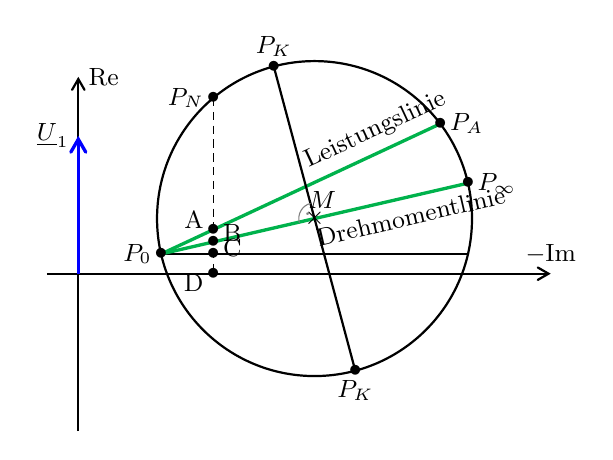
\begin{tikzpicture}[>=angle 60, font=\small]

% Koordinatensystem
\draw [->, thick] (-.4, 0) -- (6, 0) node [above] {$-$Im};
\draw [->, thick] (0, -2) -- (0, 2.5) node [right] {Re};

% Kreis
\coordinate (M) at (3, 0.7);
\draw [thick] (M) circle (2);

% Vektoren
\coordinate (U1) at (0, 1.75);
\coordinate (P0) at ($(M)+(193:2)$);
\coordinate (Pinf) at ($(P0)+(13:4)$);
\coordinate (Pa) at ($(M)+(37:2)$);
\coordinate (Pn) at ($(M)+(130:2)$);
\coordinate (H) at ($(M)+(-13:2)$);
\coordinate (D) at ($(0,0)!(Pn)!(6,0)$);

\draw [->, very thick, blue] (0, 0) -- (U1);
\draw [name path= Cline, thick] (P0) -- (H);
\draw [name path= Bline, very thick, green!70!blue] (P0) -- (Pinf) node [black, pos=0.8, below, sloped] {Drehmomentlinie};
\draw [name path= Aline, very thick, green!70!blue] (P0) -- (Pa) node [black, pos=0.8, above, sloped] {Leistungslinie};
\draw [name path= dashedline, densely dashed] (Pn) -- (D);
\draw [thick] (M) -- +(105:2) node {$\bullet$} -- +(-75:2) node {$\bullet$};
\draw [black!50!white] (M) ++(105:0.2) arc (105:195:0.2);
\draw [black!50!white] (M) ++(150:0.1) node {.};

\path [name intersections={of=Aline and dashedline, by=A}];
\path [name intersections={of=Bline and dashedline, by=B}];
\path [name intersections={of=Cline and dashedline, by=C}];

% Beschriftung
\node at (M) {$\times$};
\node at (Pinf) {$\bullet$};
\node at (P0) {$\bullet$};
\node at (Pa) {$\bullet$};
\node at (Pn) {$\bullet$};
\node at (A) {$\bullet$};
\node at (B) {$\bullet$};
\node at (C) {$\bullet$};
\node at (D) {$\bullet$};
\node at (U1) [left] {$\underline U_1$};
\node at (Pn) [left] {$P_N$};
\node at (Pa) [right] {$P_A$};
\draw (M) ++(0.1,0) node [above] {$M$};
\draw (M)++(105:2) node [above] {$P_K$};
\draw (M)++(-75:2) node [below] {$P_K$};
\draw (Pinf) node [right] {$P_\infty$};
\draw (P0)  node [left] {$P_0$};
\draw (A) +(0, 0.12) node [left] {A};
\draw (B) +(0, 0.12) node [right] {B};
\draw (C) +(0, 0.08) node [right] {C};
\draw (D) +(0, -0.12) node [left] {D};
			
\end{tikzpicture}
%!tikz source end

\end{sectionbox}

\begin{sectionbox}
\subsection{Drehmoment}
\begin{emphbox}
$M_K\sim \left(\frac{U_1}{f_1}\right)^2\qquad M_N\sim\Phi_\delta\frac{U_1}{f_1}$
\end{emphbox}
\begin{align*}
M_i = M_R + M_L + J\frac{\partial\omega}{\partial t}
\end{align*}
\subsubsection{Drehmomentgleichung}
\begin{emphbox}
\[M_i = 3p(1-\sigma)\frac{{U_1}^2}{{\omega_1}^2 L_\sigma}\frac{s \cdot s_K}{\Delta\rho_1{s_K}^2 + 2\frac{\rho_1}{\sigma}(1-\sigma)s_K s+\Delta\rho_1 s^2}\]
\end{emphbox}
Kippmoment:\\
$M_K = M_i(s_K) = \frac{3}{2} p\cdot (1-\sigma)\frac{{U_1}^2}{{\omega_1}^2 L_\sigma}\left( \frac{1}{\Delta\rho_1+\frac{\rho_1}{\sigma}(1-\sigma)}\right)$\\
$(R_1 = 0): M_K = \frac{m_1U_1\frac{I_{1Ki} - I_{10}}{2}}{2\pi\cdot n_s}$\\
Kippschlupf: $s_K = \frac{\rho_2}{\sigma}\sqrt{\frac{1+{\rho_1}^2}{1+\left(\frac{\rho_1}{\sigma}\right)^2}}$

\begin{symbolbox}
\begin{tabularx}{\columnwidth}{CC}
$s_K > 0\quad$ Motor & $s_K < 0\quad$ Generator
\end{tabularx}
\end{symbolbox}
\end{sectionbox}

\begin{sectionbox}
\subsubsection{Klossche Gleichung (Annahme $R_1 = 0$)}
\begin{emphbox}
\[\frac{M_i}{M_K} = \frac{2\cdot s_K\cdot s}{{s_K}^2 + s^2}\]
\end{emphbox}
\[s_{1,2} = s_K \frac{M_K}{M_i} \pm \sqrt{\left(s_K \frac{M_K}{M_i}\right)^2 - {s_K}^2}\]
Nur echte Lösung wenn gilt: \quad $s < s_K$
\end{sectionbox}

\begin{sectionbox}
\subsection{Symmetrische Komponenten}
\begin{symbolbox}
\begin{tabularx}{\columnwidth}{>{\centering\arraybackslash}Xc>{\centering\arraybackslash}X}
$s_m + s_g = 2$ & $s_m = s = \frac{n_s - n}{n_s}$ & $s_g = \frac{n_s + n}{n_s}$
\end{tabularx}
\end{symbolbox}

\subsubsection{Spannungen Mit- und Gegensystem}
\begin{tabular}{lc}
Mitsystem & $\underline{U}_m = \frac{1}{3}\cdot (\underline{U}_u + \underline{a}\cdot\underline{U}_v + \underline{a}^2 \cdot \underline{U}_w)$\\
Gegensystem & $\underline{U}_m = \frac{1}{3}\cdot (\underline{U}_u + \underline{a}^2\cdot\underline{U}_v + \underline{a} \cdot \underline{U}_w)$\\
Nullsystem & $\underline{U}_m = \frac{1}{3}\cdot (\underline{U}_u + \cdot\underline{U}_v + \cdot \underline{U}_w)$
\end{tabular}\\
Nullsystem verschwindet bei Dreiecksschaltung oder Sternschaltung ohne herausgeführten Sternpunkt\\

\subsubsection{Drehmoment mit Kompensation (Kippschlupf ändert sich)}
\[M_\text{ges} = M_m - M_g\]
\begin{emphbox}
\[M = 3p\cdot (1-\sigma)\cdot\frac{{U_1}^2}{{\omega}^2 L_1} \cdot\frac{\rho_2 \cdot s}{(\rho_1\cdot\rho_2 -\sigma\cdot s)^2 +(\rho_2 +s\cdot\rho_1)^2}\]
\end{emphbox}
\end{sectionbox}


\end{multicols*}
\end{document}
